\documentclass[a4paper, 12pt, openright]{book}
%\documentclass[a4paper, 12pt, openright, draft]{book}  Nalogo preverite tudi z opcijo draft, ki pokaže, katere vrstice so predolge! Pozor, v draft opciji, se slike ne pokažejo!

\usepackage[utf8]{
    inputenc
} % omogoča uporabo slovenskih črk kodiranih v formatu UTF-8
\usepackage[slovene, english]{
    babel
} % naloži, med drugim, slovenske delilne vzorce
\usepackage[pdftex]{graphicx} % omogoča vlaganje slik različnih formatov
\graphicspath{{image/}}
\usepackage{fancyhdr} % poskrbi, na primer, za glave strani
\usepackage{amssymb} % dodatni matematični simboli
\usepackage{amsmath} % eqref, npr.
\usepackage[hyphens]{url}
\usepackage{csquotes}
\usepackage[
    pdftex,
    colorlinks=true,
    citecolor=black,
    filecolor=black,
    linkcolor=black,
    urlcolor=black,
    pdfproducer={LaTeX},
    pdfcreator={LaTeX}
]{hyperref}
\usepackage{hyperxmp}

\usepackage{color}
\usepackage{soul}

\usepackage[backend=biber, style=numeric, sorting=nty,]{biblatex}

\addbibresource{literatura.bib} %Imports bibliography file

%%%%%%%%%%%%%%%%%%%%%%%%%%%%%%%%%%%%%%%%
%	DIPLOMA INFO
%%%%%%%%%%%%%%%%%%%%%%%%%%%%%%%%%%%%%%%%
\newcommand{\ttitle}{Emulacija računalnika Sinclair ZX Spectrum z vpogledom v
stanje sistema}
\newcommand{\ttitleEn}{Emulation of Sinclair ZX Spectrum computer with system
state insight}
\newcommand{\tsubject}{\ttitle}
\newcommand{\tsubjectEn}{\ttitleEn}
\newcommand{\tauthor}{Klemen Remec}
\newcommand{\tkeywords}{emulacija, Sinclair ZX Spectrum, digitalno ohranjanje}
\newcommand{\tkeywordsEn}{emulation, Sinclair ZX Spectrum, digital preservation}

%%%%%%%%%%%%%%%%%%%%%%%%%%%%%%%%%%%%%%%%
%	HYPERREF SETUP
%%%%%%%%%%%%%%%%%%%%%%%%%%%%%%%%%%%%%%%%
\hypersetup{pdftitle={\ttitle}}
\hypersetup{pdfsubject=\ttitleEn}
\hypersetup{pdfauthor={\tauthor}}
\hypersetup{pdfkeywords=\tkeywordsEn}

%%%%%%%%%%%%%%%%%%%%%%%%%%%%%%%%%%%%%%%%
% postavitev strani
%%%%%%%%%%%%%%%%%%%%%%%%%%%%%%%%%%%%%%%%

\addtolength{\marginparwidth}{-20pt} % robovi za tisk
\addtolength{\oddsidemargin}{40pt}
\addtolength{\evensidemargin}{-40pt}

\renewcommand{\baselinestretch}{1.3} % ustrezen razmik med vrsticami
\setlength{\headheight}{15pt} % potreben prostor na vrhu
\renewcommand{\chaptermark}[1]%
{\markboth{\MakeUppercase{\thechapter.\ #1}}{}}
\renewcommand{\sectionmark}[1]%
{\markright{\MakeUppercase{\thesection.\ #1}}}
\renewcommand{\headrulewidth}{0.5pt}
\renewcommand{\footrulewidth}{0pt}
\fancyhf{}
\fancyhead[LE,RO]{\sl \thepage}
%\fancyhead[LO]{\sl \rightmark} \fancyhead[RE]{\sl \leftmark}
\fancyhead[RE]{\sc \tauthor} % dodal Solina
\fancyhead[LO]{\sc Diplomska naloga} % dodal Solina

\newcommand{\BibLaTeX}{{\sc Bib}\LaTeX}
\newcommand{\BibTeX}{{\sc Bib}\TeX}

%%%%%%%%%%%%%%%%%%%%%%%%%%%%%%%%%%%%%%%%
% naslovi
%%%%%%%%%%%%%%%%%%%%%%%%%%%%%%%%%%%%%%%%

\newcommand{\autfont}{\Large}
\newcommand{\titfont}{\LARGE\bf}
\newcommand{\clearemptydoublepage}{\newpage
{\pagestyle{empty}\cleardoublepage}}
\setcounter{tocdepth}{1} % globina kazala

%%%%%%%%%%%%%%%%%%%%%%%%%%%%%%%%%%%%%%%%
% konstrukti
%%%%%%%%%%%%%%%%%%%%%%%%%%%%%%%%%%%%%%%%
\newtheorem{izrek}{Izrek}[chapter]
\newtheorem{trditev}{Trditev}[izrek]
\newenvironment{dokaz}{\emph{Dokaz.}\ }{\hspace{\fill}{$\Box$}}

%%%%%%%%%%%%%%%%%%%%%%%%%%%%%%%%%%%%%%%%%%%%%%%%%%%%%%%%%%%%%%%%%%%%%%%%%%%%%%%
%% PDF-A
%%%%%%%%%%%%%%%%%%%%%%%%%%%%%%%%%%%%%%%%%%%%%%%%%%%%%%%%%%%%%%%%%%%%%%%%%%%%%%%

%%%%%%%%%%%%%%%%%%%%%%%%%%%%%%%%%%%%%%%%
% define medatata
%%%%%%%%%%%%%%%%%%%%%%%%%%%%%%%%%%%%%%%%
\def\Title{\ttitle}
\def\Author{\tauthor, klemen.remec@gmail.com}
\def\Subject{\ttitleEn}
\def\Keywords{\tkeywordsEn}

%%%%%%%%%%%%%%%%%%%%%%%%%%%%%%%%%%%%%%%%
% \convertDate converts D:20080419103507+02'00' to 2008-04-19T10:35:07+02:00
%%%%%%%%%%%%%%%%%%%%%%%%%%%%%%%%%%%%%%%%
\def\convertDate{%
\getYear }

{\catcode`\D=12 \gdef\getYear D:#1#2#3#4{\edef\xYear{#1#2#3#4}\getMonth} }
\def\getMonth#1#2{\edef\xMonth{#1#2}\getDay}
\def\getDay#1#2{\edef\xDay{#1#2}\getHour}
\def\getHour#1#2{\edef\xHour{#1#2}\getMin}
\def\getMin#1#2{\edef\xMin{#1#2}\getSec}
\def\getSec#1#2{\edef\xSec{#1#2}\getTZh}
\def\getTZh
+#1#2{\edef\xTZh{#1#2}\getTZm}
\def\getTZm
'#1#2'{%
\edef\xTZm{#1#2}%
\edef\convDate{\xYear-\xMonth-\xDay T\xHour:\xMin:\xSec+\xTZh:\xTZm}%
}

%\expandafter\convertDate\pdfcreationdate

%%%%%%%%%%%%%%%%%%%%%%%%%%%%%%%%%%%%%%%%
% get pdftex version string
%%%%%%%%%%%%%%%%%%%%%%%%%%%%%%%%%%%%%%%%
\newcount\countA
\countA=\pdftexversion
\advance
\countA
by
-100
\def\pdftexVersionStr{pdfTeX-1.\the\countA.\pdftexrevision}

%%%%%%%%%%%%%%%%%%%%%%%%%%%%%%%%%%%%%%%%
% XMP data
%%%%%%%%%%%%%%%%%%%%%%%%%%%%%%%%%%%%%%%%
\usepackage{xmpincl}
%\includexmp{pdfa-1b}

%%%%%%%%%%%%%%%%%%%%%%%%%%%%%%%%%%%%%%%%
% pdfInfo
%%%%%%%%%%%%%%%%%%%%%%%%%%%%%%%%%%%%%%%%
\pdfinfo{%
/Title (\ttitle) /Author (\tauthor, klemen.remec@gmail.com) /Subject (\ttitleEn) /Keywords (\tkeywordsEn) /ModDate (\pdfcreationdate) /Trapped /False }

%%%%%%%%%%%%%%%%%%%%%%%%%%%%%%%%%%%%%%%%
% znaki za copyright stran
%%%%%%%%%%%%%%%%%%%%%%%%%%%%%%%%%%%%%%%%

\newcommand{\CcImageCc}[1]{%

\includegraphics[scale=#1]{cc_cc_30.pdf}%
}
\newcommand{\CcImageBy}[1]{%

\includegraphics[scale=#1]{cc_by_30.pdf}%
}
\newcommand{\CcImageSa}[1]{%

\includegraphics[scale=#1]{cc_sa_30.pdf}%
}

%%%%%%%%%%%%%%%%%%%%%%%%%%%%%%%%%%%%%%%%%%%%%%%%%%%%%%%%%%%%%%%%%%%%%%%%%%%%%%%
%%%%%%%%%%%%%%%%%%%%%%%%%%%%%%%%%%%%%%%%%%%%%%%%%%%%%%%%%%%%%%%%%%%%%%%%%%%%%%%

\begin{document}
    \selectlanguage{slovene}
    \frontmatter
    \setcounter{page}{1} %
    \renewcommand{\thepage}{} % preprečimo težave s številkami strani v kazalu

    %%%%%%%%%%%%%%%%%%%%%%%%%%%%%%%%%%%%%%%%
    %naslovnica
    \thispagestyle{empty}%
    \begin{center}
        {\large\sc Univerza v Ljubljani\\%


        %      Fakulteta za elektrotehniko\\% za študijski program Multimedija


        %      Fakulteta za upravo\\% za študijski program Upravna informatika
        Fakulteta za računalništvo in informatiko\\%


        %      Fakulteta za matematiko in fiziko\\% za študijski program Računalništvo in matematika
        } \vskip 10em%
        {\autfont \tauthor\par}%
        {\titfont \ttitle \par}%
        {\vskip 3em \textsc{DIPLOMSKO DELO\\[5mm] UNIVERZITETNI ŠTUDIJSKI PROGRAM\\ PRVE STOPNJE\\ RAČUNALNIŠTVO IN INFORMATIKA}\par}
        \vfill
        \null%
        % izberite pravi habilitacijski naziv mentorja!
        {\large \textsc{Mentor}: izr. prof. dr. Jurij Mihelič\par}%
        %${\large \textsc{Somentor}:  viš. pred./doc./izr. prof./prof. dr.  Martin Krpan \par}%
        {\vskip 2em \large Ljubljana, \the\year \par}%
    \end{center}
    % prazna stran
    %\clearemptydoublepage
    % izjava o licencah itd. se izpiše na hrbtni strani naslovnice

    %%%%%%%%%%%%%%%%%%%%%%%%%%%%%%%%%%%%%%%%
    %copyright stran
    %%%%%%%%%%%%%%%%%%%%%%%%%%%%%%%%%%%%%%%%
    \newpage
    \thispagestyle{empty}

    \vspace*{5cm}
    {\small \noindent To delo je ponujeno pod licenco \textit{Creative Commons Priznanje avtorstva-Deljenje pod enakimi pogoji 2.5 Slovenija} (ali novej\v so razli\v cico). To pomeni, da se tako besedilo, slike, grafi in druge sestavine dela kot tudi rezultati diplomskega dela lahko prosto distribuirajo, reproducirajo, uporabljajo, priobčujejo javnosti in predelujejo, pod pogojem, da se jasno in vidno navede avtorja in naslov tega dela in da se v primeru spremembe, preoblikovanja ali uporabe tega dela v svojem delu, lahko distribuira predelava le pod licenco, ki je enaka tej. Podrobnosti licence so dostopne na spletni strani \href{http://creativecommons.si}{creativecommons.si} ali na Inštitutu za intelektualno lastnino, Streliška 1, 1000 Ljubljana.

    \vspace*{1cm} \begin{center}% 0.66 / 0.89 = 0.741573033707865
    \CcImageCc{0.741573033707865}\hspace*{1ex}\CcImageBy{1}\hspace*{1ex}\CcImageSa{1}%
    \end{center} }

    \vspace*{1cm}
    {\small \noindent Izvorna koda diplomskega dela, njeni rezultati in v ta namen razvita programska oprema je ponujena pod licenco GNU General Public License, različica 3 (ali novejša). To pomeni, da se lahko prosto distribuira in/ali predeluje pod njenimi pogoji. Podrobnosti licence so dostopne na spletni strani \url{http://www.gnu.org/licenses/}. }

    \vfill
    \begin{center}
        \ \\
        \vfill
        {\em Besedilo je oblikovano z urejevalnikom besedil \LaTeX.}
    \end{center}

    % prazna stran
    \clearemptydoublepage

    %%%%%%%%%%%%%%%%%%%%%%%%%%%%%%%%%%%%%%%%
    % stran 3 med uvodnimi listi
    \thispagestyle{empty}
    \

    \vfill

    \bigskip
    \noindent
    \textbf{Kandidat:} Klemen Remec\\
    \noindent
    \textbf{Naslov:} Emulacija računalnika Sinclair ZX Spectrum z vpogledom v
    stanje sistema\\
    % vstavite ustrezen naziv študijskega programa!
    \noindent
    \textbf{Vrsta naloge:} Diplomska naloga na univerzitetnem programu prve
    stopnje Računalništvo in informatika \\
    % izberite pravi habilitacijski naziv mentorja!
    \noindent
    \textbf{Mentor:} izr. prof. dr. Jurij Mihelič\\
    %\noindent\textbf{Somentor:} isto kot za mentorja

    \bigskip
    \noindent
    \textbf{Opis:}\\ Besedilo teme diplomskega dela študent prepiše iz
    študijskega informacijskega sistema, kamor ga je vnesel mentor. V nekaj
    stavkih bo opisal, kaj pričakuje od kandidatovega diplomskega dela. Kaj so
    cilji, kakšne metode naj uporabi, morda bo zapisal tudi ključno literaturo.

    \bigskip
    \noindent
    \textbf{Title:} Emulation of Sinclair ZX Spectrum computer with system state insight

    \bigskip
    \noindent
    \textbf{Description:}\\ opis diplome v angleščini

    \vfill

    \vspace{2cm}

    % prazna stran
    \clearemptydoublepage

    % zahvala
    \thispagestyle{empty}
    \mbox{}
    \vfill
    \null\it%
    \noindent
    Na tem mestu zapišite, komu se zahvaljujete za pomoč pri izdelavi diplomske naloge
    oziroma pri vašem študiju nasploh. Pazite, da ne boste koga pozabili.
    Utegnil vam bo zameriti. Temu se da izogniti tako, da celotno zahvalo
    izpustite. \rm\normalfont

    % prazna stran
    \clearemptydoublepage

    %%%%%%%%%%%%%%%%%%%%%%%%%%%%%%%%%%%%%%%%
    % kazalo
    \pagestyle{empty}
    \def\thepage{}% preprečimo težave s številkami strani v kazalu
    \tableofcontents
    {}

    % prazna stran
    \clearemptydoublepage

    %%%%%%%%%%%%%%%%%%%%%%%%%%%%%%%%%%%%%%%%
    % seznam kratic

    \chapter*{Seznam uporabljenih kratic}

    \noindent
    \begin{tabular}{p{0.12\textwidth}|p{.37\textwidth}|p{.43\textwidth}}
        {\bf kratica} & {\bf angleško}                                     & {\bf slovensko}                                            \\
        \hline
        {\bf ASCII}   & American Standard Code for Information Interchange & ameriški standardni kod za izmenjavo informacij            \\
        {\bf BASIC}   & Beginners' All-purpose Symbolic Instruction Code   & programski jezik BASIC                                     \\
        {\bf CPE}     & central processing unit                            & centralna procesna enota                                   \\
        {\bf CRC}     & cyclic redundancy check                            & ciklično preverjanje redundance                            \\
        {\bf EAR}     & earphone                                           & vhod za signal iz kasetofona                               \\
        {\bf IFF}     & interrupt flip-flop                                & prekinitveni preklopnik                                    \\
        {\bf INT}     & interrupt                                          & maskabilna prekinitev                                      \\
        {\bf KMP}     & Kotlin Multiplatform                               & večplatformska tehnologija Kotlin Multiplatform            \\
        {\bf LIFO}    & last in, first out                                 & oblika delovanja sklada po principu zadnji noter, prvi ven \\
        {\bf MIC}     & microphone                                         & izhod za signal proti kasetofonu                           \\
        {\bf NMI}     & non-maskable interrupt                             & nemaskabilna prekinitev                                    \\
        {\bf PC}      & program counter                                    & programski števec                                          \\
        {\bf PDF/A}   & Portable Document Format/Archive                   & arhivska različica zapisa PDF                              \\
        {\bf PSP}     & interrupt handler                                  & prekinitveno-servisni program                              \\
        {\bf RAM}     & random access memory                               & bralno-pisalni pomnilnik                                   \\
        {\bf ROM}     & read-only memory                                   & bralni pomnilnik                                           \\
        {\bf SNA}     & snapshot                                           & posnetek stanja emulatorja                                 \\
        {\bf SP}      & stack pointer                                      & kazalec sklada                                             \\
        {\bf TAP}     & tape                                               & zapis standardnih kasetnih blokov                          \\
        {\bf TZX}     & ZX tape                                            & datotečni format zapisa kasete za ZX Spectrum              \\
        {\bf ULA}     & uncommitted logic array                            & logično vezje ULA                                          \\
        {\bf V/I}     & input/output                                       & vhod/izhod                                                 \\
    \end{tabular}

    % prazna stran
    \clearemptydoublepage

    %%%%%%%%%%%%%%%%%%%%%%%%%%%%%%%%%%%%%%%%
    % povzetek
    \phantomsection
    \addcontentsline{toc}{chapter}{Povzetek}
    \chapter*{Povzetek}

    \noindent
    \textbf{Naslov:} \ttitle
    \bigskip

    \noindent
    \textbf{Avtor:} \tauthor
    \bigskip

    %\noindent\textbf{Povzetek:}
    \noindent
    V vzorcu je predstavljen postopek priprave diplomskega dela z uporabo okolja
    \LaTeX. Vaš povzetek mora sicer vsebovati približno 100 besed, ta tukaj je
    odločno prekratek. Dober povzetek vključuje: (1) kratek opis obravnavanega
    problema, (2) kratek opis vašega pristopa za reševanje tega problema in (3) (najbolj
    uspešen) rezultat ali prispevek diplomske naloge.

    \bigskip

    \noindent
    \textbf{Ključne besede:} \tkeywords.
    % prazna stran
    \clearemptydoublepage

    %%%%%%%%%%%%%%%%%%%%%%%%%%%%%%%%%%%%%%%%
    % abstract
    \phantomsection \selectlanguage{english}
    \addcontentsline{toc}{chapter}{Abstract}
    \chapter*{Abstract}

    \noindent
    \textbf{Title:} \ttitleEn
    \bigskip

    \noindent
    \textbf{Author:} \tauthor
    \bigskip

    %\noindent\textbf{Abstract:}
    \noindent
    This sample document presents an approach to typesetting your BSc thesis
    using \LaTeX. A proper abstract should contain around 100 words which makes this
    one way too short.
    \bigskip

    \noindent
    \textbf{Keywords:} \tkeywordsEn. \selectlanguage{slovene}
    % prazna stran
    \clearemptydoublepage

    %%%%%%%%%%%%%%%%%%%%%%%%%%%%%%%%%%%%%%%%
    \mainmatter
    \setcounter{page}{1}
    \pagestyle{fancy}

    \chapter{Uvod}

    ZX Spectrum, viden na sliki \ref{wikipediazxspectrum_pic1}, je 8-bitni
    domači računalnik podjetja Sinclair Research, ki je v osemdesetih letih pomembno
    zaznamoval evropski trg mikroračunalnikov in postal dostopen širokemu krogu domačih
    uporabnikov.

    \begin{figure}[htb]
        \begin{center}
            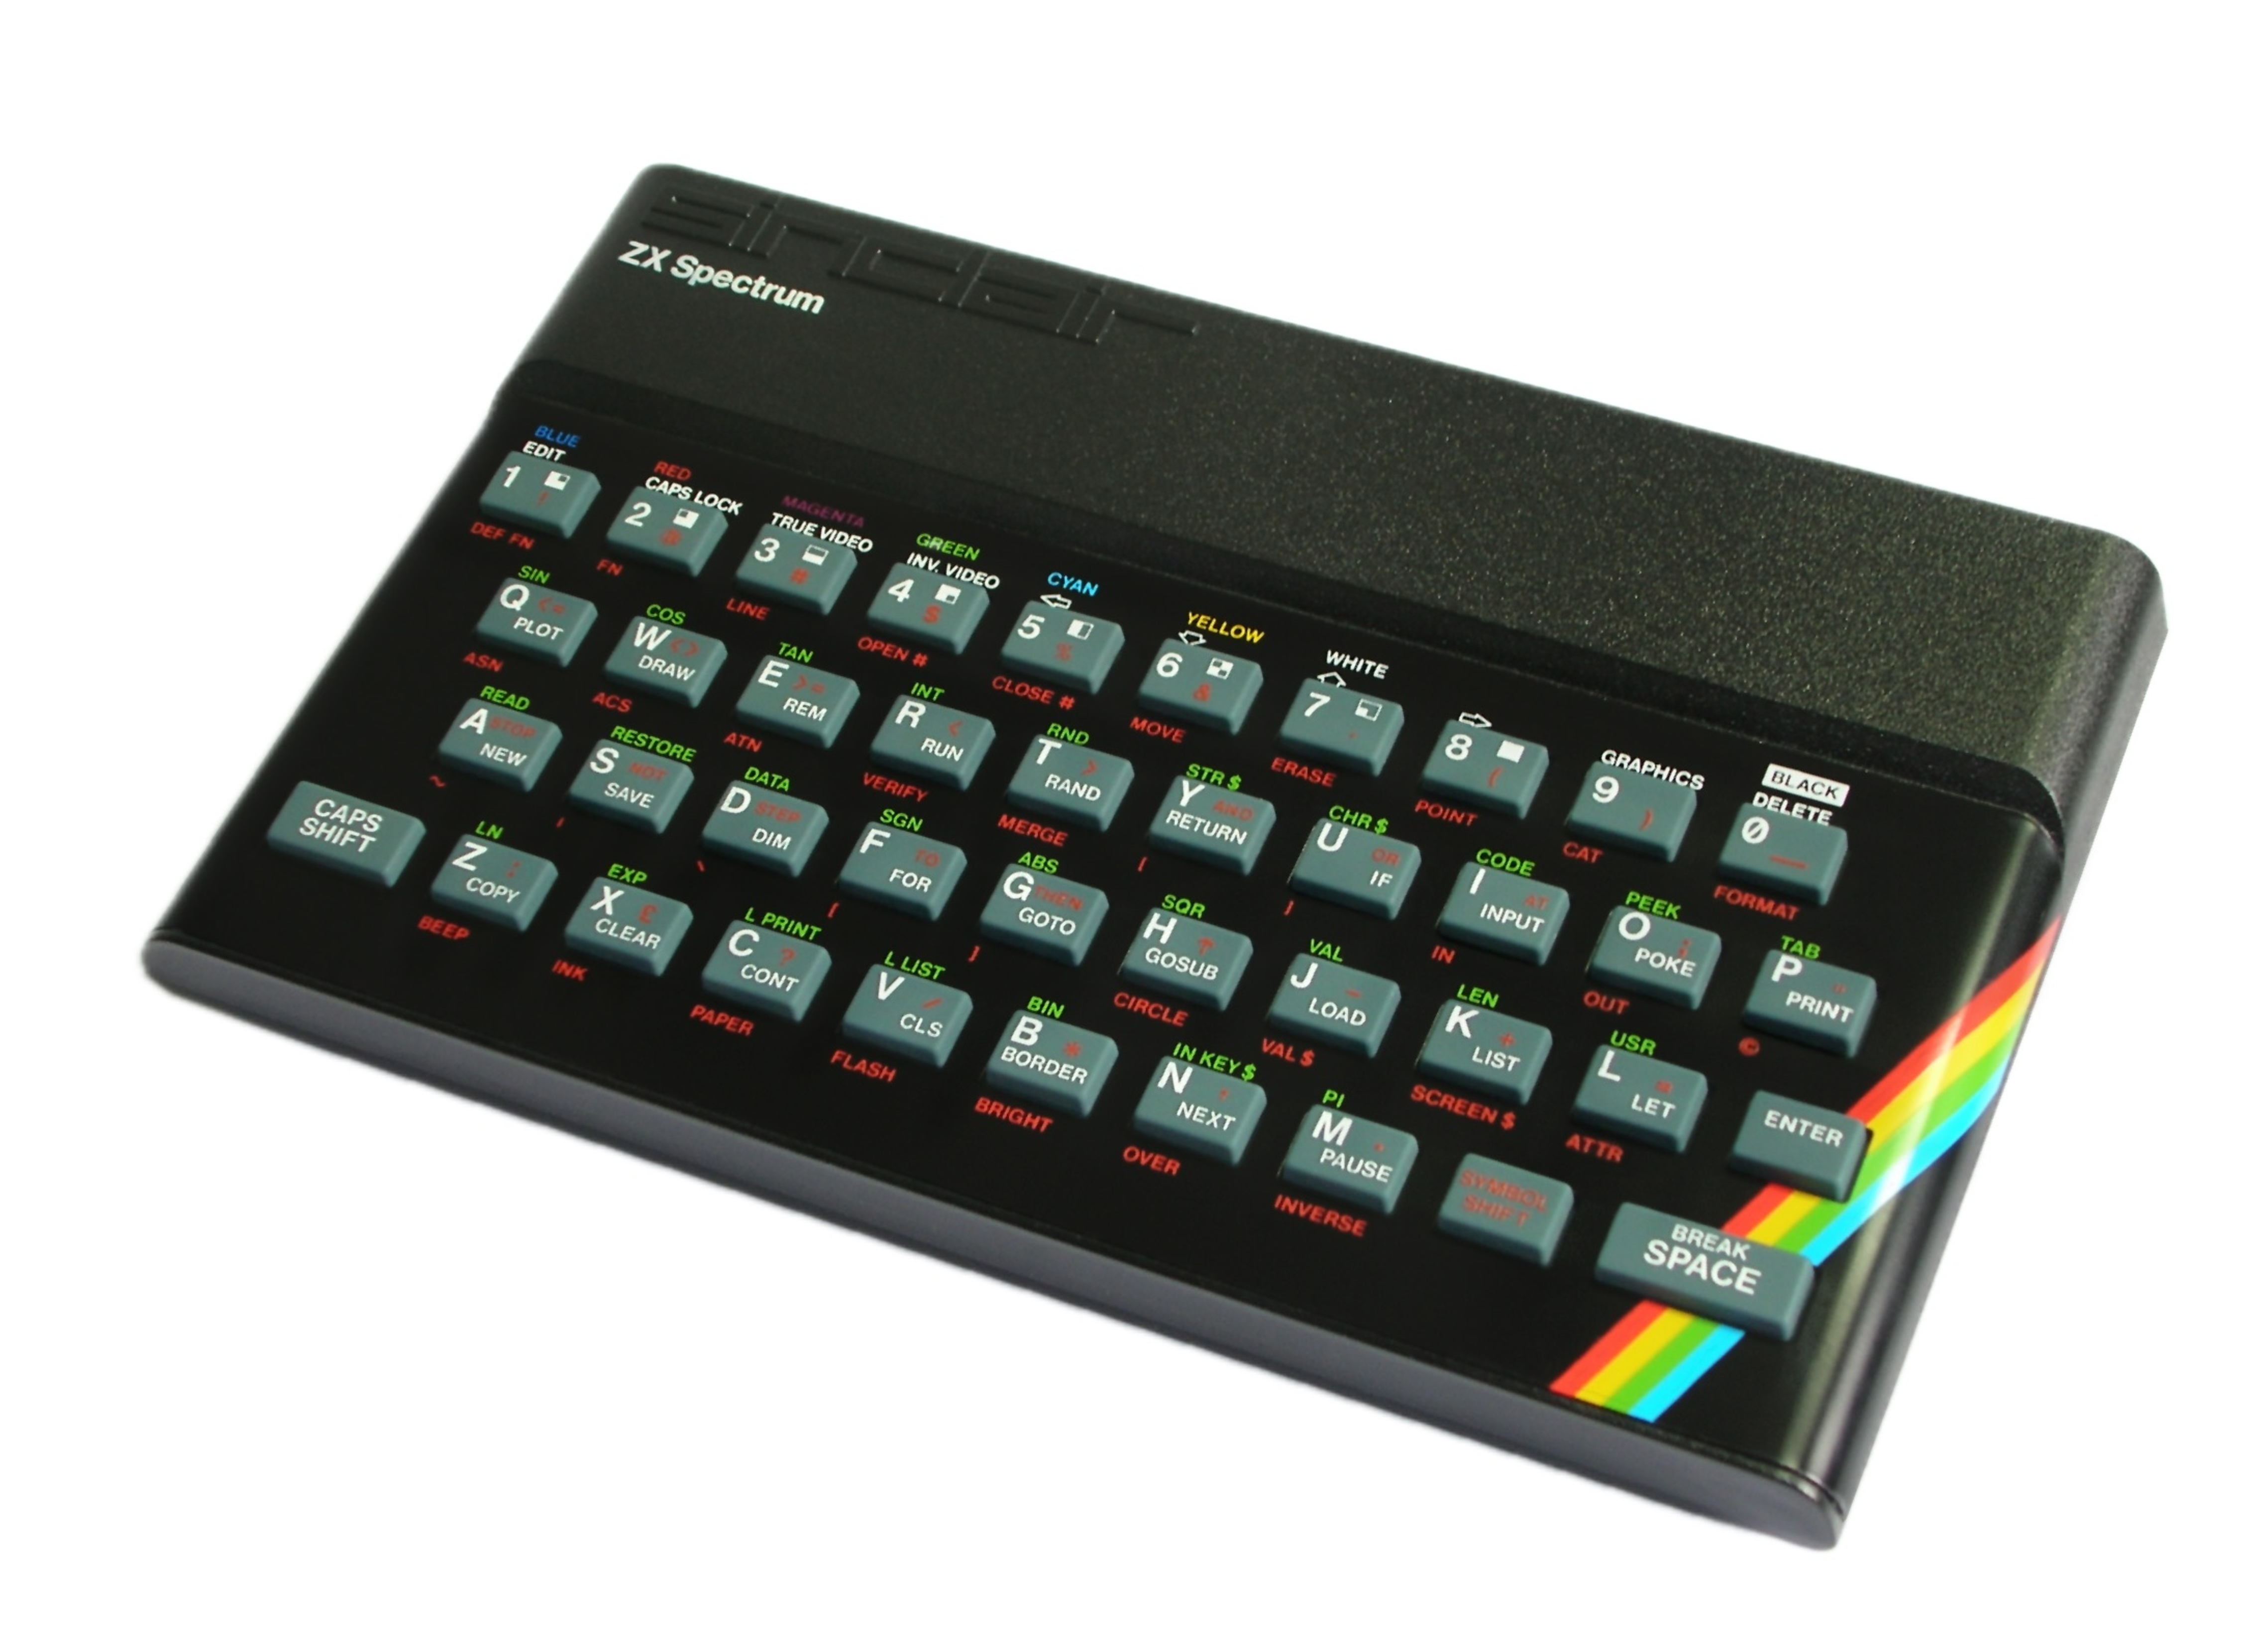
\includegraphics[width=0.6\textwidth]{wikipediazxspectrum_pic1}
        \end{center}
        \caption{Računalnik ZX Spectrum 48K. ~\cite{wikipediazxspectrum}}
        \label{wikipediazxspectrum_pic1}
    \end{figure}

    Namen diplomskega dela je razviti delujoč emulator in razhroščevalnik
    sistema ZX Spectrum 48K. Emulator mora podpirati poganjanje programov,
    napisanih za Spectrum in razhroščevanje z vpogledom v notranje stanje
    sistema. Zaradi poudarka na razhroščevanju mora pri tem omogočati pregled in spreminjanje
    vrednosti registrov ter pomnilnika, pregled in razlago pomena naloženih
    ukazov in delov pomnilnika. Tak vpogled ni pomemben le za boljše razumevanje sistema,
    temveč tudi za ohranjanje znanja o njegovem delovanju. Delovanje emulatorja se
    ovrednoti z zagonom nekaj izbranih programov in iger, s čimer potrdimo
    pravilno delovanje emulacije.

    V nadaljnjih poglavjih je najprej predstavljen računalnik ZX Spectrum, njegov
    vpliv na slovensko in svetovno okolje ter pomen ohranjanja takega znanja.
    Sledi opis splošne zgradbe emulatorja, zatem pa poglavja o zasnovi in implementaciji
    posameznih delov sistema, to so pomnilnik, procesor Z80 in ULA, ki obravnava
    časovnik, zaslon, tipkovnico, kasete in zvok.

    \chapter{ZX Spectrum}
    \label{zxspectrum}

    \section{Zgodovina podjetja Sinclair in računalnikov ZX Spectrum}

    Sinclair Research je pred ZX Spectrumom že uveljavil nizkocenovne domače
    računalnike, kot sta ZX80 in ZX81, ki sta poleg računalnika ZX Spectruma
    videna na sliki \ref{i4cysinclairomputers_pic1}. Bila sta bila namenjena predvsem
    učenju programiranja in prvi uporabi računalnika doma. ZX Spectrum je bil
    predstavljen aprila 1982 kot zmogljivejši naslednik ZX81, napram kateremu je na
    trg prinesel barvno grafiko, višjo ločljivost zaslonske slike, zvok in bolj razvito
    podporo okolju BASIC ~\cite{sinclairstory}.

    \begin{figure}[htb]
        \begin{center}
            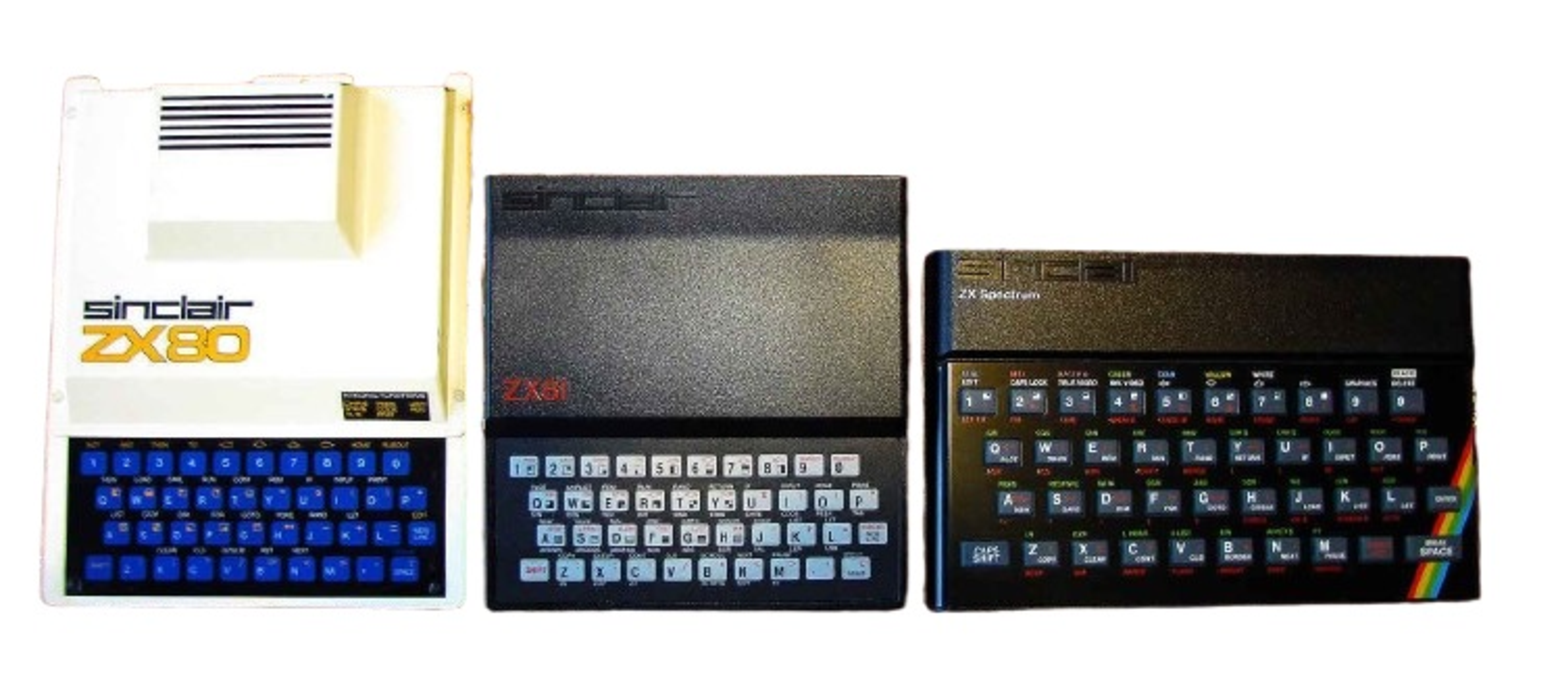
\includegraphics[width=0.7\textwidth]{i4cysinclairomputers_pic1}
        \end{center}
        \caption{Računalniki Sinclair ZX80, ZX81 in ZX Spectrum. ~\cite{i4cysinclairomputers}}
        \label{i4cysinclairomputers_pic1}
    \end{figure}

    Prvotni Spectrum je bil na voljo v različicah s 16 KB in 48 KB RAMa, obe pa
    sta uporabljali procesor Zilog Z80 in 16 KB ROMa. Računalnik se je dalo priključiti
    na navaden televizor, programe pa je praviloma nalagal s kasete, kar je pomembno
    vplivalo na način uporabe in razširjanja programske opreme. Zaradi nizke
    cene in velike programske knjižnice je Spectrum postal eden
    najprepoznavnejših evropskih domačih računalnikov osemdesetih let ~\cite{zxspectrumintroduction}
    ~\cite{sinclairstory}.

    Družina ZX Spectrum se je pozneje širila z različnimi modeli. Spectrum+ je
    obdržal tehnično osnovo modela 48K, vendar jo je prestavil v večje ohišje z izboljšano
    tipkovnico, poznejši Spectrum 128 pa je razširil pomnilnik na 128 KB, dogradil
    implementacijo okolja BASIC, izboljšal zvočni čip in dodal možnosti za
    priklop zunanjih naprav. Ker je model 48K predstavljal osrednjo in najbolj razširjeno
    različico Spectruma ter osnovo za velik del Spectrumove programske opreme,
    se prav zato nadaljnja obravnava in implementacija emulatorja osredotočata
    na ta model ~\cite{sinclairstory} ~\cite{zxspectrum128introduction}.

    \subsection{Vpliv na slovenski trg mikroračunalnikov in Jakopin}

    V slovenskem prostoru je bil ZX Spectrum pomemben predvsem kot cenovno dostopen
    domači računalnik. Prvi Spectrumi so se pri nas pojavili sredi leta 1982, kmalu
    zatem pa naj bi jih bilo samo v Ljubljani že nekaj tisoč. Njegova
    priljubljenost je bila povezana z nizko ceno in velikim številom iger, vendar
    se uporaba ni ustavila le pri zabavi ~\cite{mojmikroines1984}.

    Takšno okolje je pomembno za razumevanje pomena programa INES Primoža
    Jakopina. Program ni bil le uporabniški pripomoček, temveč primer doma
    razvite programske opreme, ki je iz Spectruma, takrat večinoma uporabljanega
    za igranje iger, naredila delovno orodje. INES je bil januarja 1985
    objavljen kot kasetni program, ki je omogočal obdelavo besedil spremeljive dolžine
    (primer delovanja je viden na sliki \ref{subspectrum_ines}), slik ter
    manjših podatkovnih zbirk. Podpora šumnikom in jugoslovanskim črkam je bila posebej
    pomembna za domačo rabo ~\cite{mojmikroines1984} ~\cite{mojmikroines1985saje}
    ~\cite{mojmikroines1985jakopin}.

    \begin{figure}[htb]
        \begin{center}
            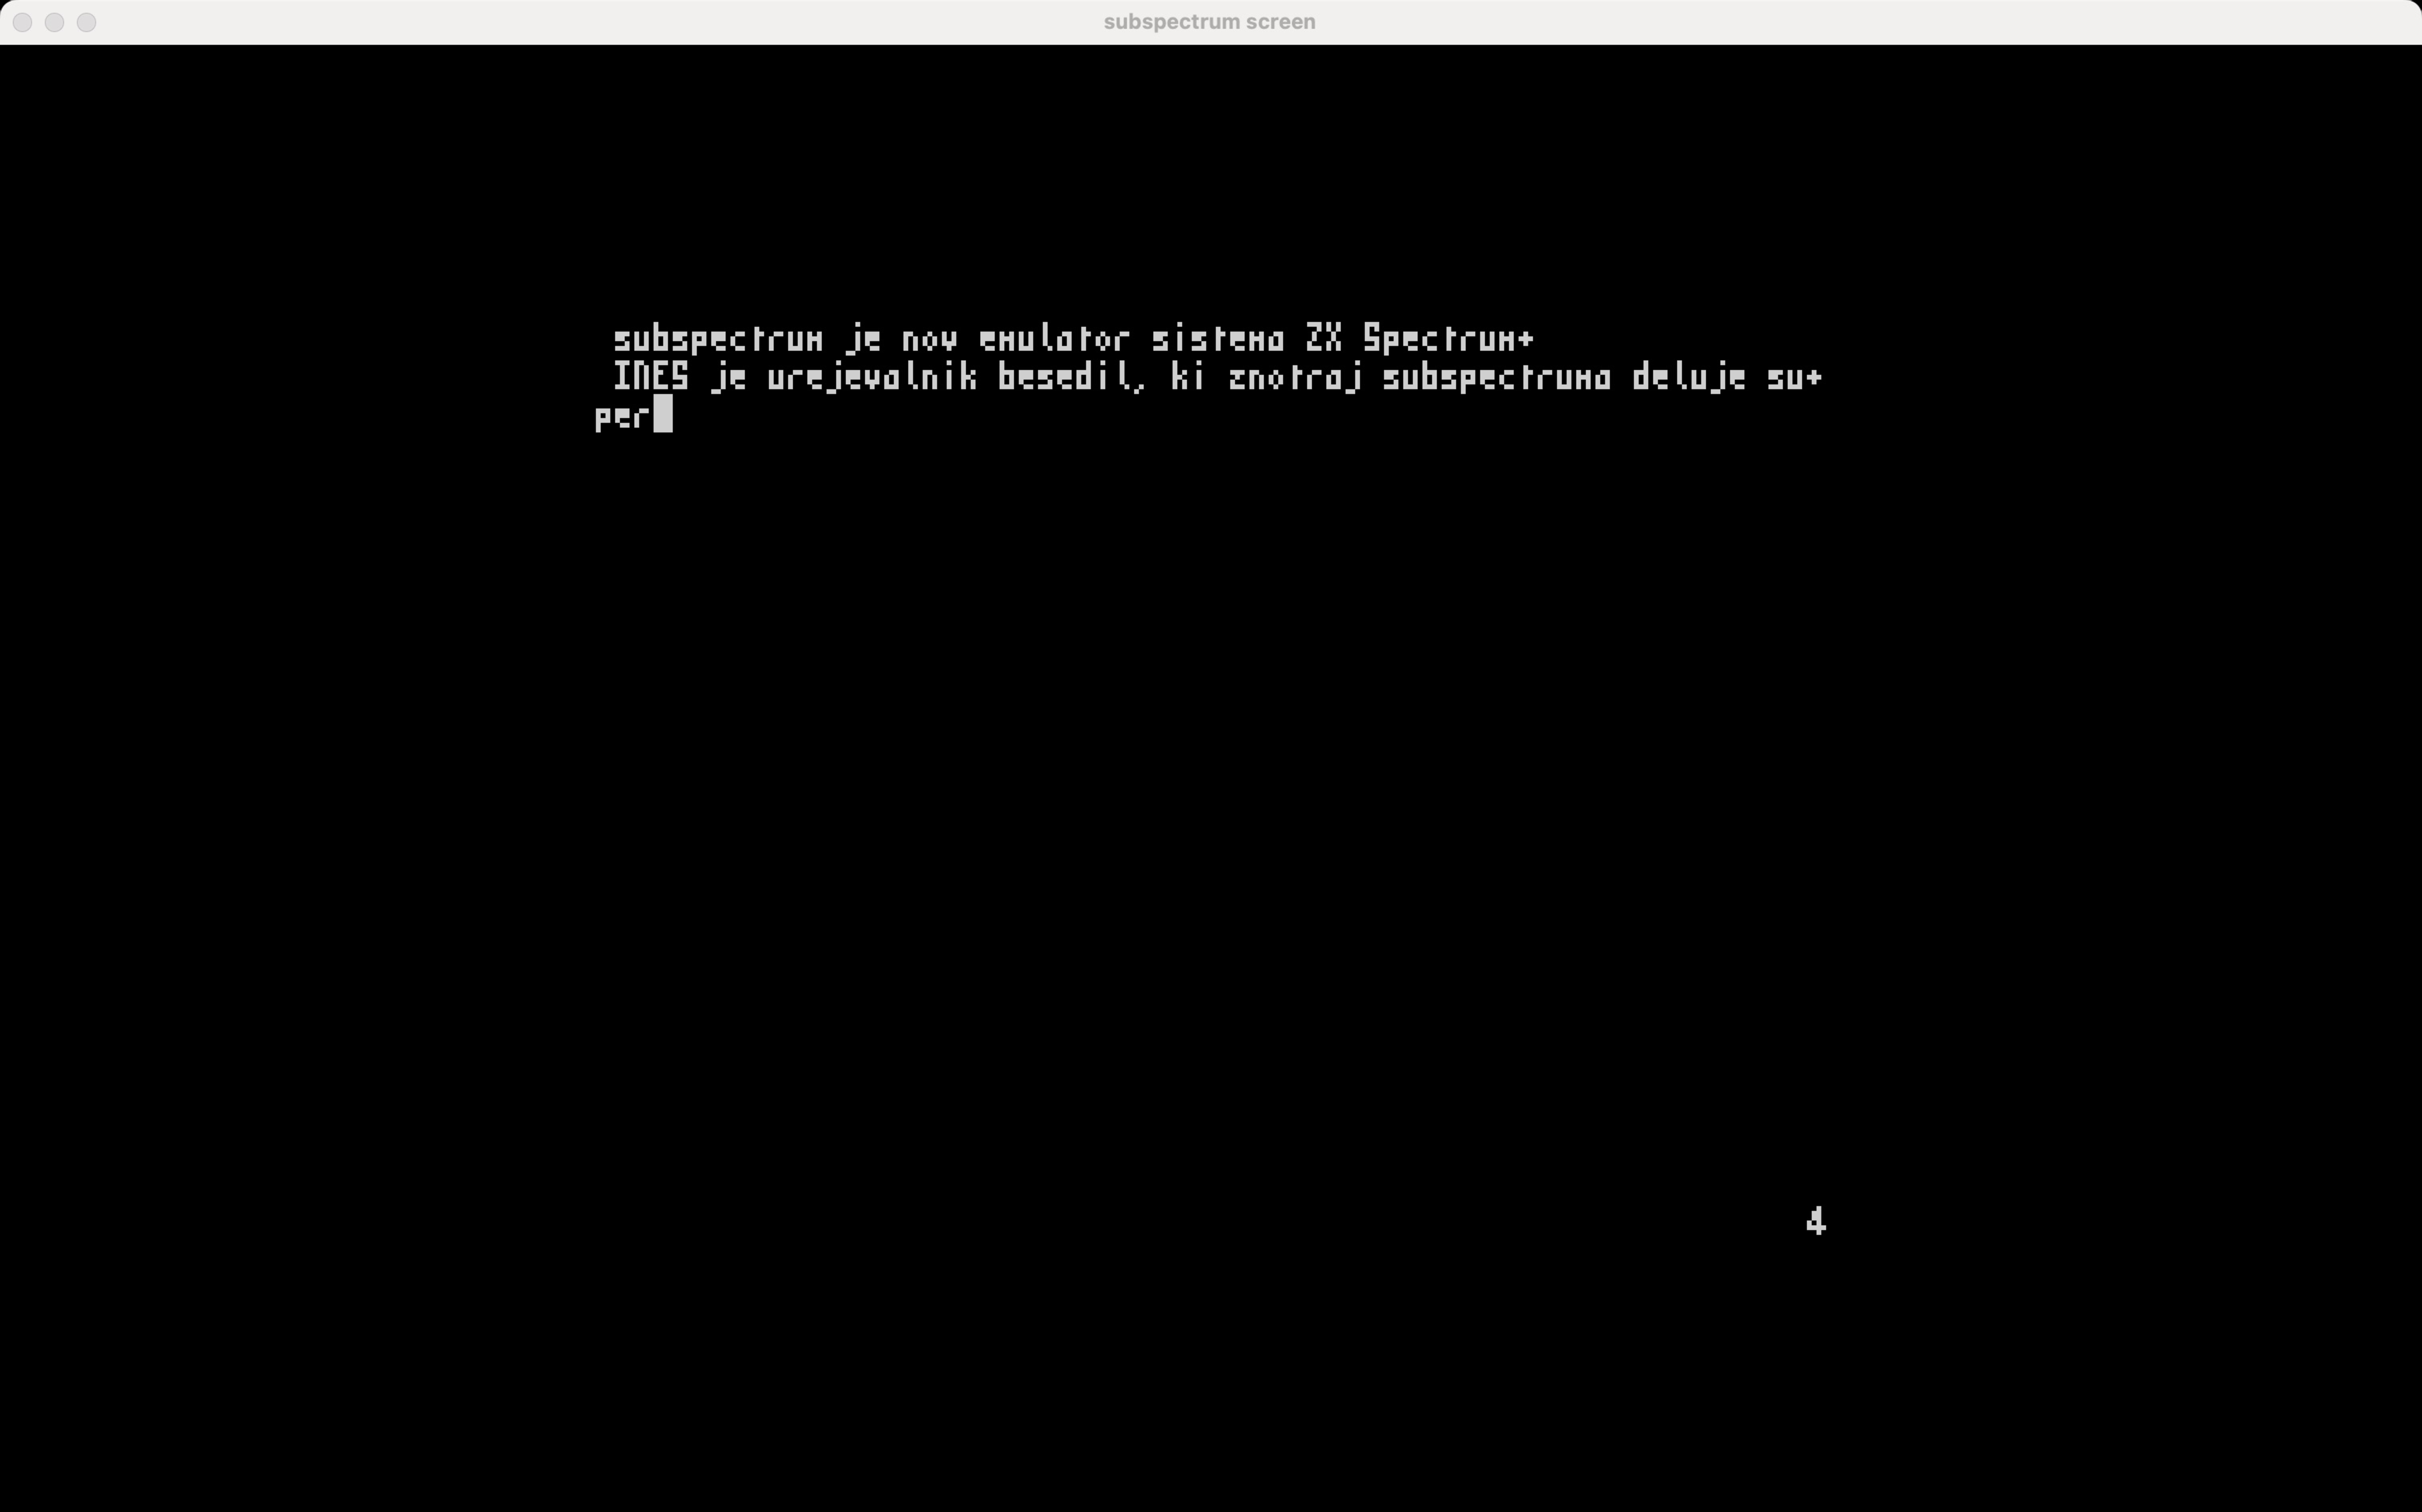
\includegraphics[width=0.7\textwidth]{subspectrum_ines}
        \end{center}
        \caption{Prikaz delovanja urejanja besedila v programu INES znotraj
        razvitega emulatorja.}
        \label{subspectrum_ines}
    \end{figure}

    Tehnično je z INES pokazal, kje so bile postavljene meje učinkovitosti
    BASICa za uporabo v zahtevnejših programih - iskanje po besedilu je bilo v
    BASICu bistveno počasnejše napram implementaciji v strojnem jeziku. Ta premik
    od tolmačenega BASICa proti programiranju v strojnem jeziku se je poznal skozi
    vso razvojno pot programov od TESS, BESS do INES, ter kasneje programov STEVE
    za Atari ST in EVA za modernejše osebne računalnike ~\cite{jakopininessteveeva}
    ~\cite{jakopinines} ~\cite{jakopinsteve} ~\cite{mojmikroines1984}.

    \subsection{Pomen ohranjanja računalniških sistemov in programske opreme
    prek emulacije}

    Ohranjanje celotne programske dediščine ZX Spectruma in drugih sistemov ni
    vezano le na shranjeni kasetni zapis programov, temveč tudi na konkretno izvajalno
    okolje: procesor, pomnilnik, ROM, način nalaganja, tipkovnico, prikaz na zaslonu
    in druge lastnosti sistema. Digitalno ohranjanje zato zajema tudi
    računalniške sisteme in programsko opremo kot digitalne artefakte, katerih dostopnost
    je odvisna od hitro spreminjajočih se nosilcev podatkov, formatov, programov in
    strojne opreme ~\cite{mihelicferleemulacija}.

    Računalniška emulacija pomeni programsko posnemanje drugega računalniškega
    sistema. Za ohranjanje programov je pomembno posnemanje delovanja notranjih komponent
    sistema in vhodno-izhodnih naprav, možnost uporabe sistema preko nalaganja
    programov, vnosa podatkov in prikaza rezultatov. Emulacija tako ohranja
    digitalni artefakt skupaj z zadostnim delom njegovega izvajalnega in
    uporabniškega okolja ~\cite{mihelicferleemulacija}.

    \section{Pregled strojne opreme}

    \subsection{Kratek pregled strojne opreme}

    Računalnik ZX Spectrum ima na zadnji strani več vtičnic in priključkov:
    vtičnico 9V DC IN, ki se prek napajalne enote priključi v električno omrežje,
    3,5 milimeterska vtičnica EAR, ki se lahko poveže z izhodno vtičnico za slušalke
    ali zvočnik na kasetofonu, 3,5 milimeterska vtičnica MIC, ki se poveže z vhodno
    vtičnico za mikrofon na kasetofonu, vtičnico za televizijo in robni
    priključek za povezavo z dodatno opremo. Povezave med osnovnimi deli sistema so
    videne na sliki \ref{zxspectrumintroduction_pic1} ~\cite{zxspectrumintroduction}.

    Ko računalnik ugasnemo, se vse v njem shranjene informacije izgubijo, če jih
    pred tem ne prenesemo na zunanji medij, kot je na primer kaseta. Če se
    kadarkoli zapletemo pri uporabi računalnika, ga lahko le izključimo iz električnega
    omrežja in nazaj vklopimo, ter tako ponastavimo brez skrbi poškodbe
    računalniku ~\cite{zxspectrumintroduction}.

    \begin{figure}[htb]
        \begin{center}
            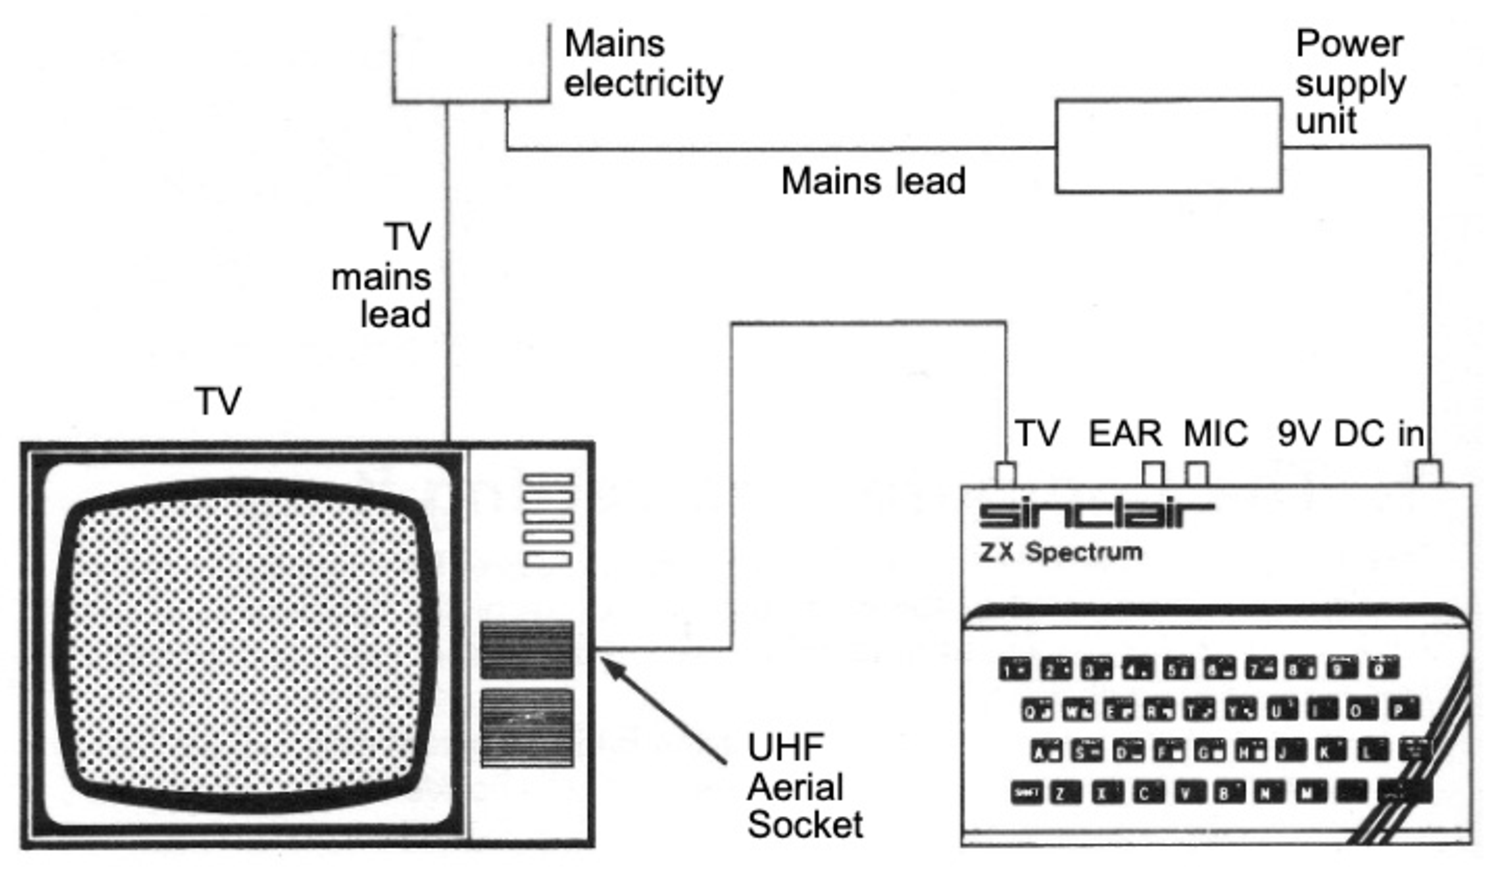
\includegraphics[width=0.7\textwidth]{zxspectrumintroduction_pic1}
        \end{center}
        \caption{Skica povezav komponent sistema \cite{zxspectrumintroduction}.}
        \label{zxspectrumintroduction_pic1}
    \end{figure}

    Razporeditev glavnih notranjih komponent računalnika je videna na sliki
    \ref{zxspectrumintroduction_pic2}.

    CPE Z80 predstavlja možgane računalnika, ki nadzira vse operacije, izvaja
    aritmetične račune, sprejema odločitve in na splošno upravlja, kaj naj
    računalnik naredi ~\cite{zxspectrumintroduction}.

    ROM vsebuje 16384 zlogov (16K) navodil v strojnem kodu Z80, ki sestavljajo
    osnovni program računalnika, in procesorju narekuje, kaj naj stori v vseh
    predvidljivih okoliščinah. Ta program je edinstven za ZX Spectrum. ~\cite{zxspectrumintroduction}

    RAM obsega osem čipov za shranjevanje podatkov, ki jih procesor želi obdržati,
    kot so programi v BASICu, spremenljivke, slika za televizijski zaslon in
    različni elementi, ki spremljajo stanje računalnika. ~\cite{zxspectrumintroduction}.

    ULA deluje kot komunikacijski center sistema, ki poskrbi, da se vse, kar
    zahteva procesor, tudi dejansko izvede, hkrati pa bere pomnilnik za sestavo
    televizijske slike in pošilja ustrezne signale televizijskemu vmesniku ~\cite{zxspectrumintroduction}.

    PAL kodirnik je skupina komponent, ki pretvarja televizijski izhod iz
    logičnega čipa v obliko, primerno za barvne televizije ~\cite{zxspectrumintroduction}.

    Regulator napetosti pretvarja rahlo nestabilno napetost napajanja v
    popolnoma konstantnih pet voltov za zanesljivo delovanje sistema ~\cite{zxspectrumintroduction}.

    UHF/VHF modulator prenaša sliko na televizijski zaslon ~\cite{zxspectrumintroduction}.

    Zvočnik predstavlja zvočni izhod za zvok ~\cite{zxspectrumintroduction}.

    \begin{figure}[htb]
        \begin{center}
            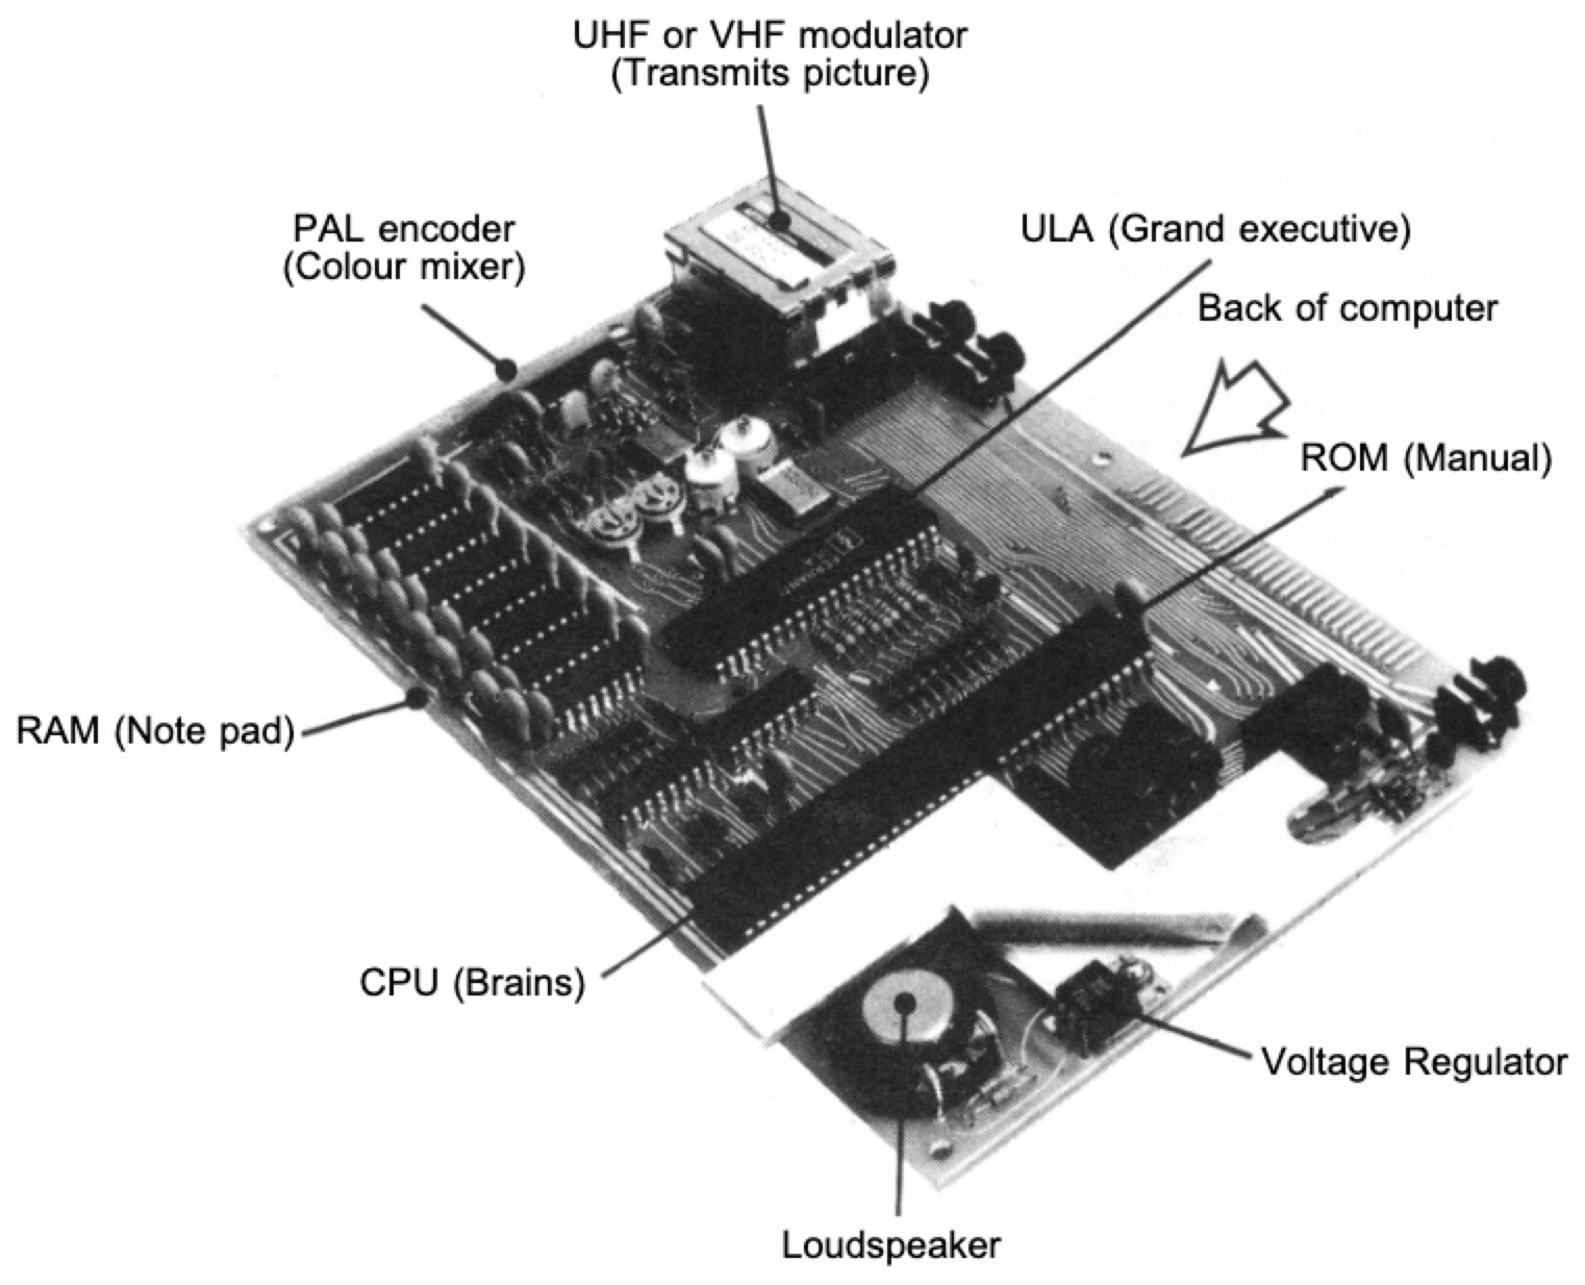
\includegraphics[width=0.7\textwidth]{zxspectrumintroduction_pic2}
        \end{center}
        \caption{Skica notranjih komponent računalnika ZX Spectrum ~\cite{zxspectrumintroduction}.}
        \label{zxspectrumintroduction_pic2}
    \end{figure}

    \subsection{Ostala dodatna oprema}
    Obstaja še druga oprema, ki se lahko uporabi s Spectrumom ~\cite{zxspectrumbasicprogramming}.

    ZX Microdrive je naprava za hitro množično shranjevanje in je veliko bolj
    prilagodljiva pri načinu uporabe kot kasetni snemalnik ~\cite{zxspectrumbasicprogramming}.

    Omrežni priključek se uporablja za povezovanje več računalnikov ZX Spectrum,
    da lahko med seboj komunicirajo ~\cite{zxspectrumbasicprogramming}.

    Vmesnik RS232 omogoča standardno povezavo računalnika s tipkovnicami,
    tiskalniki, računalniki in drugimi zunanjimi napravami, tudi če niso bili
    zasnovani posebej za Spectrum ~\cite{zxspectrumbasicprogramming}.

    \section{Pregled in primerjava z obstoječimi emulatorji}

    Obstaja veliko število emulatorjev računalnika ZX Spectrum, ki se razlikujejo
    po namenu. Nekateri so namenjeni predvsem udobnemu poganjanju iger in
    programov, drugi čim natančnejši emulaciji različnih modelov in zunanjih naprav,
    tretji pa vgradnji emulacije v spletne strani ali razvojnemu delu. Tako je,
    poleg zmožnosti zagona poljubnega programa, pomembno tudi razlikovanje v podpori
    različnih modelov računalnika ZX Spectrum, podpora različnim datotečnim
    formatom, natančnost emulacije ter možnosti vpogleda v notranje stanje sistema.

    Med najbolj uveljavljenimi emulatorji sta Fuse in Spectaculator. Fuse je
    odprtokodni emulator s podporo vseh večjih operacijskih sistemov in je
    primer splošnega emulatorja z zelo široko združljivostjo: podpira več modelov
    Spectruma, sorodne računalnike, številne formate datotek in dodatno opremo.
    Spectaculator je komercialni emulator, pri katerem je večji poudarek na uporabniški
    izkušnji: udobnem nalaganju programov, virtualnem kasetofonu, shranjevanju
    stanja in pripravljenosti za igranje na osebnih računalnikih ter mobilnih
    napravah. Posebno skupino predstavljajo spletni emulatorji, na primer
    JSSpeccy 3, kjer je glavna prednost izvajanje neposredno v brskalniku, zato
    so primerni za enostavnejše predstavitve programov brez namestitve
    samostojne aplikacije ~\cite{fuseemulator} ~\cite{spectaculator} ~\cite{jsspeccy3}.

    Obstoječi zreli emulatorji so večinoma namenjeni široki združljivosti,
    udobni uporabi in podpori velikemu številu modelov, formatov ter dodatnih naprav.
    Emulator, razvit v okviru tega diplomskega dela, po obsegu ni namenjen
    neposredni zamenjavi teh rešitev. Omejen je na najpopularnejši model ZX Spectrum
    48K in na dele sistema, ki so potrebni za poganjanje tipičnih programov: procesor
    Z80, pomnilnik, ULA, zaslon, tipkovnico, zvok ter nalaganje kasetnih datotek.
    Njegova posebnost je pregleden razhroščevalni pregled notranjega stanja sistema,
    ki ponuja vpogled v vrednosti registrov, pomnilnika in v pomnilnik naloženih razstavljenih
    ukazov, lažji pregled namembnosti posameznih delov pomnilnika, ROMa in posameznih
    ukazov znotraj ROMa, izvajanju naloženega programa po korakih, prekinitvenih točkah,
    in drugih pripomočkov za lažje razumevanje delovanja originalnega sistema.

    \section{Programiranje emulatorja in razhroščevalnika}

    Emulator je razvit kot aplikacija, ki poleg samega izvajanja programov
    omogoča vpogled in posege tudi v notranje stanje emuliranega računalnika. Zato
    posamezni deli sistema niso skriti za emulacijsko zanko, ampak so
    implementirani kot ločeni modeli komponent delujočega sistema: registri,
    pomnilnik, V/I vrata, časovnik ter ostale naprave in funkcionalnosti
    računalnika. Procesor vrednosti stanja teh modelov spreminja med izvajanjem ukazov,
    uporabniški vmesnik pa jih opazuje in prikaže v razhroščevalniku.

    \subsection{Uporabljene tehnologije}

    Projekt uporablja ogrodje Kotlin Multiplatform, ki se uporablja za za
    ustvarjanje aplikacij s skupno kodo za različna izvajalna okolja, na primer namizne,
    spletne in mobilne aplikacije. V emulatorju se ta zmožnost uporablja predvsem
    tako, da sta skupna emulacijska logika in večina uporabniškega vmesnika
    definirana v skupnem modulu, platformno odvisni deli, kot sta izbira datotek
    in zvočni izhod, pa v ločenih modulih.

    Uporabniški vmesnik je narejen s knjižnico Compose Multiplatform. Z njo so
    implementirana podokna za registre, pomnilnik in razstavljene ukaze, orodna
    vrstica in ločeno okno zaslona. Daljši tek procesorja se izvaja asinhrono v ozadju,
    uporabniški vmesnik pa se posodobi le ob spremembah stanja. Gradnjo,
    izvajanje testov in pripravo namiznih paketov se izvaja preko orodja Gradle.

    \subsection{Kratek pregled delovanja emulacije in vpogleda v sistem}

    Na sliki \ref{subspectrum_interface} vidimo primer vmesnika emulatorja.
    Podokno za registre prikazuje vrednosti splošnih in posebnih registrov ter
    zastavic, podokno za pomnilnik prikazuje vrednosti pomnilniških lokacij po naslovih,
    podokno z razstavljenimi ukazi pa prikazuje ukaze, dekodirane iz trenutne vsebine
    pomnilnika. Grafični izhod emuliranega računalnika je prikazan v ločenem
    oknu zaslona. Ko procesor ne teče, lahko uporabnik neposredno spremeni
    vrednosti registrov, pomnilniških celic in ukaznih zlogov.

    Iz orodne vrstice lahko uporabnik ponovno naloži ROM ali kasetni program,
    ponastavi stanje sistema, izvede posamezen procesorski korak, ki izvede
    trenutni ukaz, zažene in ustavi tek procesorja, v katerem se ti koraki
    ponavljajo do zaustavitve ali prekinitvene točke, preklopi hitrost izvajanja emulacije,
    odpre okno zaslona ter nastavi način tipkovnice in omogoči zvok.

    \begin{figure}[htb]
        \begin{center}
            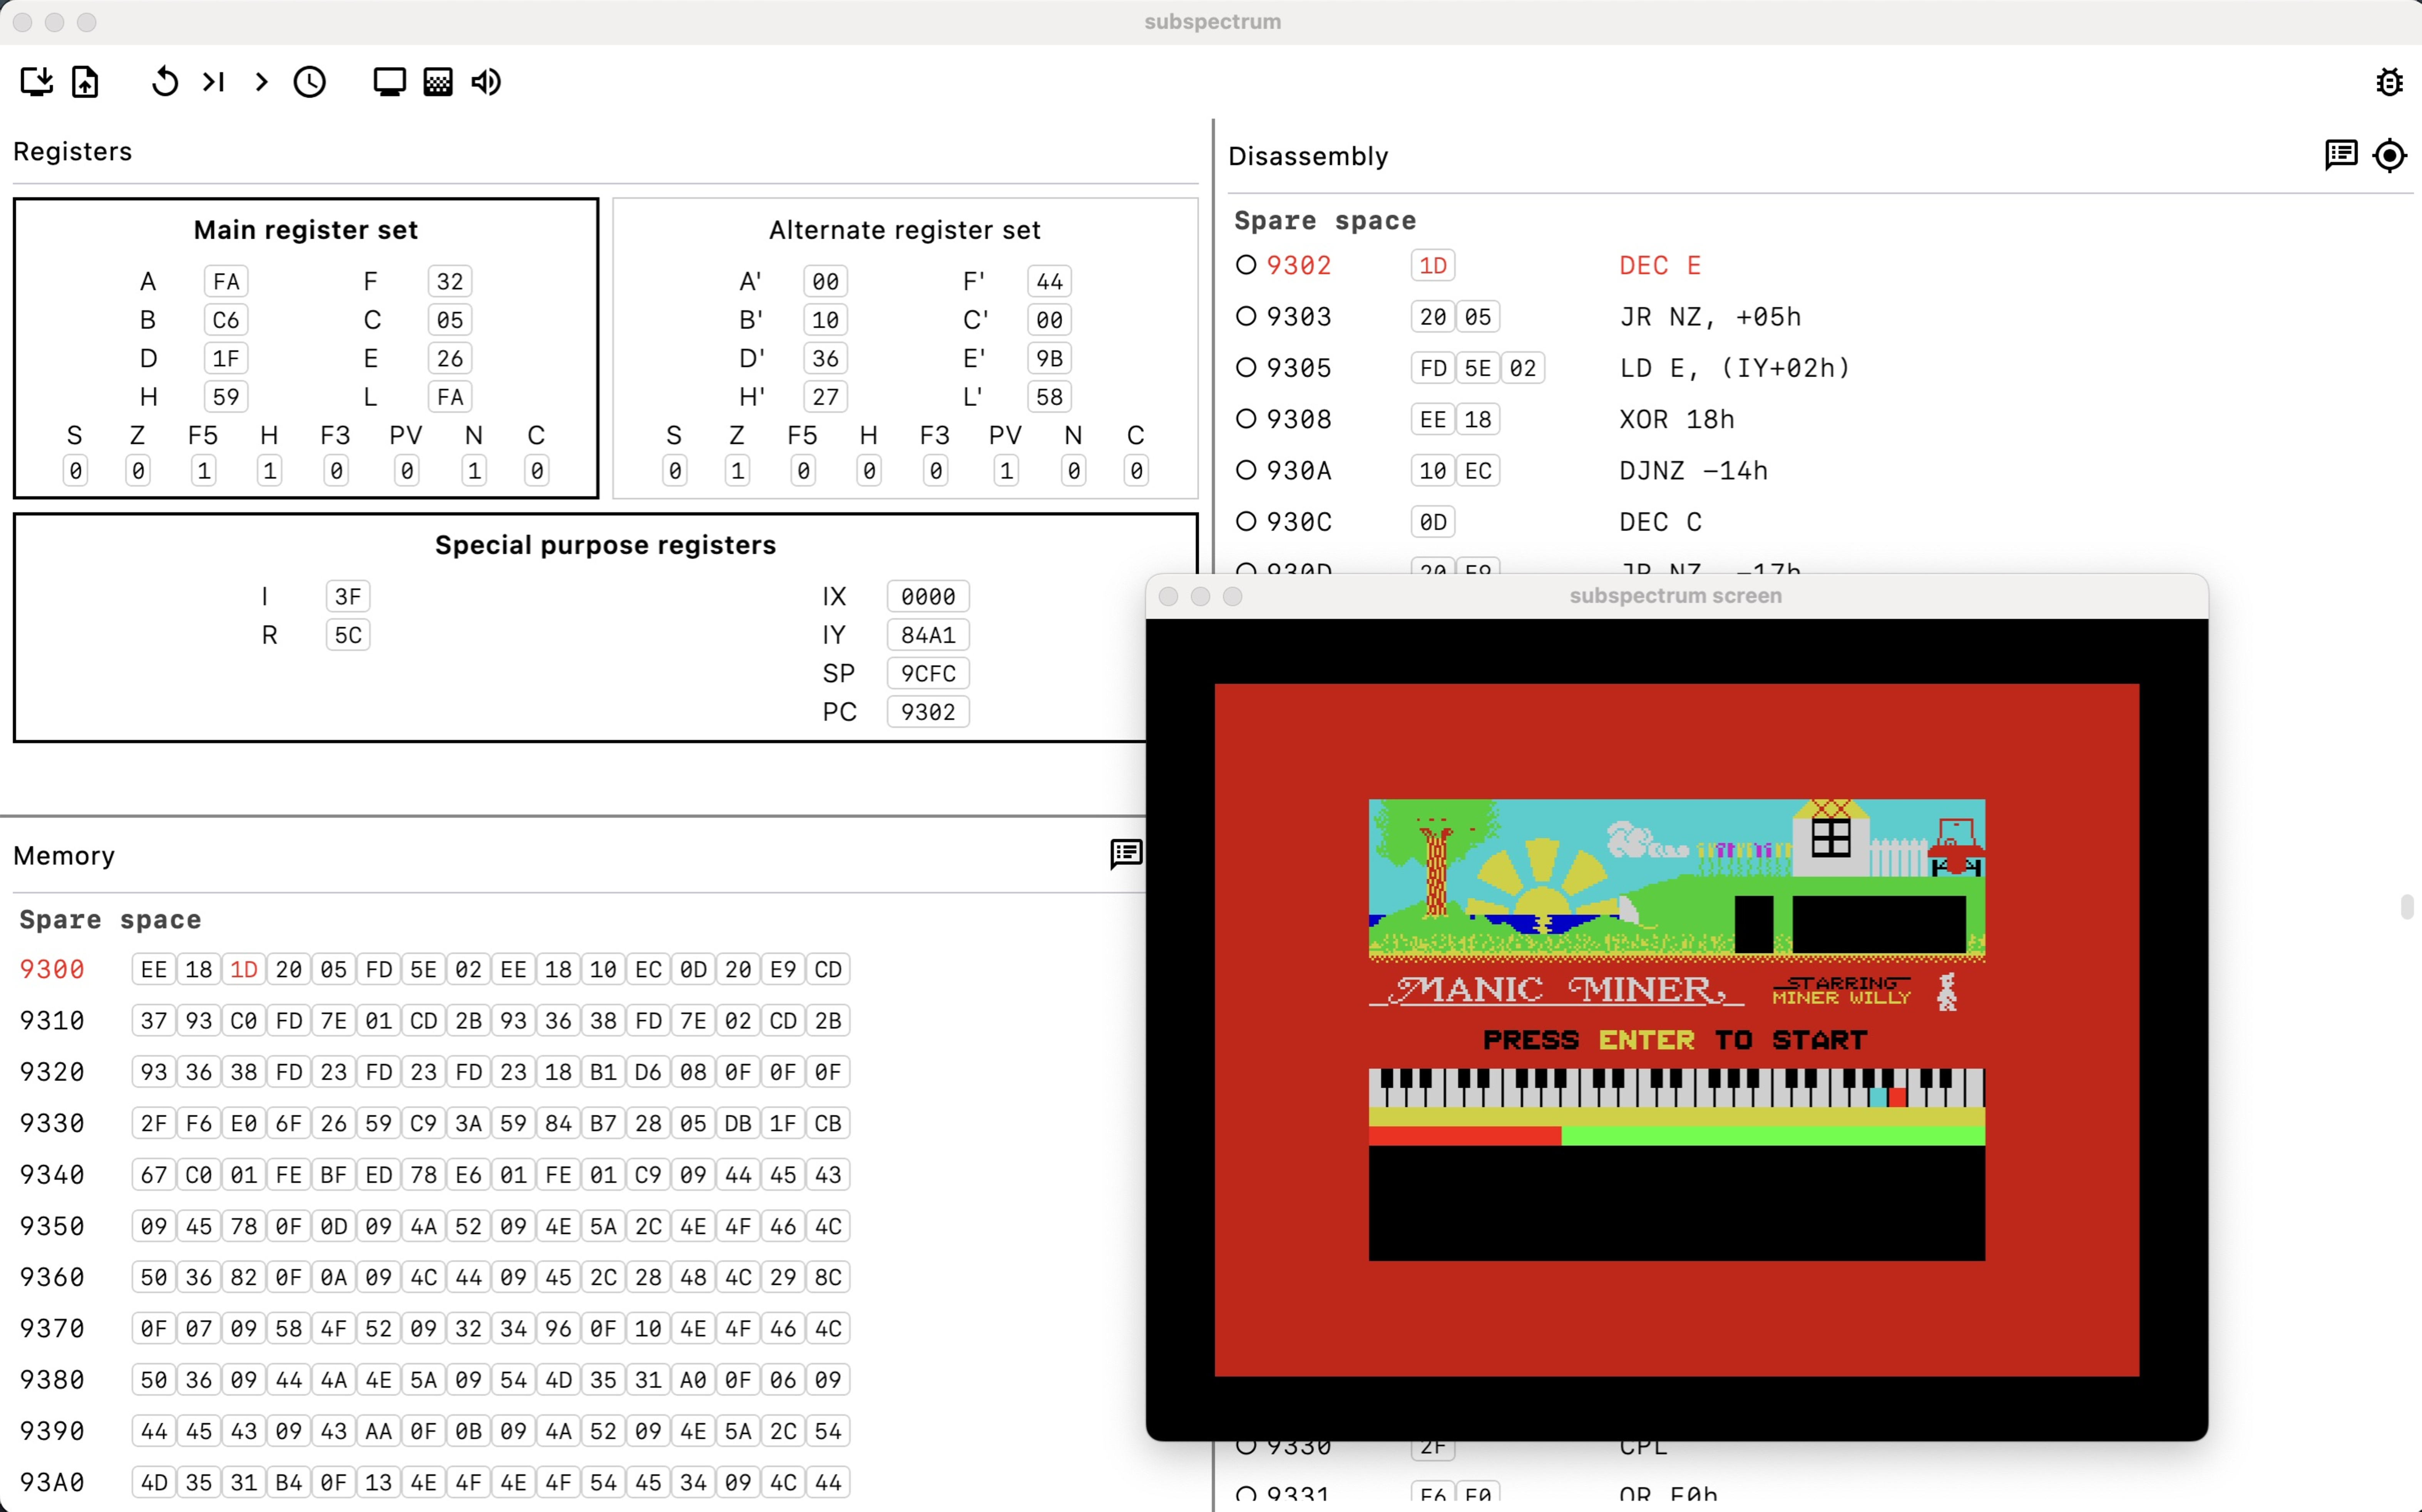
\includegraphics[width=0.7\textwidth]{subspectrum_interface}
        \end{center}
        \caption{Posnetek zaslona ob uporabi razvitega emulatorja.}
        \label{subspectrum_interface}
    \end{figure}

    Ob zagonu emulator najprej ponastavi stanje sistema in v pomnilnik naloži izbrani
    ROM. Osrednji del izvajanja je metoda \texttt{Processor.step}. Ta prebere
    ukaz na naslovu programskega števca, ga dekodira, premakne programski števec,
    izvede učinek ukaza in posodobi vrednost časovnika glede na dolžino izvajanja
    ukaza.

    \chapter{Pomnilnik}
    \label{pomnilnik}

    Pomnilnik hrani podatke v obliki zlogov (vredosti med 0 in 255), ki se
    nahajajo na dvozložnih pomnilniških naslovih med \texttt{0x0000} in \texttt{0xFFFF}.
    ~\cite{zxspectrumbasicprogramming}

    \section{Razdelitev delov pomnilnika in njihov pomen}

    V računalniku ZX Spectrum je pomnilnik razdeljen na ROM, ki se nanaša na naslovni
    prostor med \texttt{0x0000} in \texttt{0x3FFF}, ter RAM, ki se nanaša na naslovni
    prostor med \texttt{0x4000} in \texttt{0xFFFF} ~\cite{zxspectrumbasicprogramming}.

    Branje vrednosti iz pomnilnika deluje pri delu s podatki v ROMu in RAMu, pisanje
    vrednosti v pomnilnik pa deluje le v RAMu (ukaz pisanja v ROM se bo izvedel, a
    brez učinka) ~\cite{strojnijezikzaprocesorz80}.

    RAM je nadalje razdeljen na območja z različnimi nameni uporabe, pomembnejša
    območja pa so sledeča ~\cite{zxspectrumbasicprogramming} ~\cite{strojnijezikzaprocesorz80}:
    \begin{itemize}
        \item zaslonska datoteka vsebuje podatke za prikaz vsebine na zaslon,

        \item atributi položajev znakov hranijo informacije o prikazu zaslona,

        \item medpomnilnik tiskalnika hrani znake, ki jih mora tiskalnik
            natisniti, kadar pa tiskalnika ne uporabljamo, ostaja ta prostor
            neizkoriščen,

        \item sistemske spremenljivke vsebujejo razne informacije o stanju računalnika,

        \item sistem BASIC vsebuje uporabniški program v BASICu, njegove
            spremeljivke in druge podatke ter sklad za aritmetični kalkulator, in
            se razteza do naslova, na katerega kaže sistemska spremenljivka
            RAMTOP,

        \item prosti pomnilnik je zavarovan pred vplivi programa v BASICu in pred
            posegi nadzornega programa,

        \item strojni sklad, ki se začenja 2 zloga pod vrhom prostega pomnilnika,
            uporablja procesor Z80,

        \item računski sklad predstavlja 30 zlogov velik prostor z začetkom na naslovu,
            shranjenem v sistemski spremenljivki MEMBOT, ki se uporablja za računske
            operacije v plavajoči vejici,

        \item definicije uporabniško definiranih grafičnih znakov.
    \end{itemize}

    Pri vnosu več podatkov v dano območje, kot je njegova privzeta velikost, se
    ostala območja premaknejo navzgor, in obratno pri brisanju podatkov ~\cite{zxspectrumbasicprogramming}.

    \section{ROM}

    V ROMu shranjen nadzorni program poleg pravilnega zagona opravlja tudi mnoge druge
    naloge osnovnega delovanja sistema, kot so izrisovanje slike na zaslon, spremljanje
    pritiskov tipk, tolmačenje pognanega programa v BASICu in posredovanje napak
    o njegovem izvajanju, delo s plavajočo vejico, itd ~\cite{zxspectrumintroduction}
    ~\cite{strojnijezikzaprocesorz80}.

    Procesor ne pozna sintakse in pravil izvajanja BASICa. Programe v BASICu zato
    berejo in izvajajo ROMovi podprogrami v strojnem jeziku, strojni programi, tako
    nadzorni program ROMa kot uporabniški strojni programi, pa se izvajajo
    neposredno na procesorju ~\cite{strojnijezikzaprocesorz80}.

    \section{Sistemske spremenljivke}
    Zlogi na pomnilniških naslovih med \texttt{0x5C00} in \texttt{0x5CB5} se uporabljajo
    za hrambo in spreminjanje informacij o stanju oziroma delovanju sistema ~\cite{zxspectrumbasicprogramming}.

    Bolj pomembne sistemske spremenljivke so sledeče ~\cite{zxspectrumbasicprogramming}
    ~\cite{strojnijezikzaprocesorz80}:
    \begin{itemize}
        \item VARS na naslovu \texttt{0x5C4B}, ki vsebuje naslov začetka spremenljivk
            programa BASIC,

        \item PROG na naslovu \texttt{0x5C53}, ki vsebuje naslov začetka programa
            v BASICu,

        \item E\_LINE na naslovu \texttt{0x5C59}, ki vsebuje naslov konca programa
            v BASICu,

        \item RAMTOP na naslovu \texttt{0x5CB2}, ki vsebuje naslov zadnjega zloga
            sistema BASIC,

        \item P-RAMT na naslovu \texttt{0x5CB4}, ki vsebuje naslov zadnjega zloga
            fizičnega pomnilnika,

        \item BORDCR na naslovu \texttt{0x5C48}, katerih prvi trije biti definirajo
            barvo obrobe zaslona,

        \item FRAMES na naslovih \texttt{0x5C78}-\texttt{0x5C7A}, ki vsebuje 3-zložni
            števec prikazanih slikovnih okvirov, ki se pri evropskem video standardu
            poveča vsakih 20 ms oziroma vsako 1/50 sekunde. Števec je bolj
            natančen kot naivna programska implementacija, vendar se začasno ustavi
            med spuščanjem zvoka oziroma operacijami s kasetofonom, tiskalnikom
            in drugimi zunanjimi, zaradi česar izgublja na natančnosti.

        \item ATTR\_P na naslovu \texttt{0x5C8D}, ki vsebuje definicije uporabljanih
            barv papirja in papirja, ter drugih atributov stalnega prikaza
            znakov,

        \item CHARS na naslovu \texttt{0x5C36}, ki vsebuje naslov začetka definicije
            nabora znakov.
    \end{itemize}

    \section{Implementacija v emulatorju}

    Ker model ZX Spectrum 48K ne uporablja preklapljanja pomnilniških bank, je
    pomnilnik v emulatorju predstavljen kot en sam 64 KB velik naslovni prostor. Pomnilniški
    naslov je implementiran kot 16-bitna vrednost \texttt{UShort}, vsebina pomnilnika
    pa kot polje zlogov. Polje je ovito v pomožni razred \texttt{DataByteArray},
    ki poleg dostopa do posameznih zlogov omogoča tudi kopiranje obsegov in
    oblikovan heksadecimalni izpis.

    Osrednji razred za delo s pomnilnikom je \texttt{MemorySet}. Ta vsebuje
    metode za branje in pisanje ene celice, branje in pisanje zaporednega bloka celic
    ter branje in nastavljanje posameznega bita. Nad njim je definiran objekt
    \texttt{Memory}, ki vsebuje skupno instanco razreda \texttt{MemorySet}. Zato
    procesor, ULA, nalaganje kaset in uporabniški vmesnik ne hranijo ločenih
    kopij pomnilnika, ampak vsi dostopajo do istega stanja emuliranega računalnika.
    Procesor iz njega bere ukazne zloge, operande in podatke, ULA pa iz območij
    \texttt{0x4000}-\texttt{0x57FF} in \texttt{0x5800}-\texttt{0x5AFF} bere
    podatke zaslonske datoteke in atributov.

    Meja med ROMom in RAMom je v emulatorju določena s konstanto \texttt{ROM\_END\_ADDRESS},
    katere vrednost je \texttt{0x3FFF}. Metodi \texttt{setMemoryCell} in \texttt{setMemoryCells}
    zato pri običajnem izvajanju ne spremenita celic v območju ROMa. Pri zapisu enega
    zloga se tak zapis preprosto prezre, pri zapisu večjega bloka pa metoda
    zapiše samo del bloka, ki pade v območje RAMa. S tem se ohrani obnašanje
    pravega računalnika, kjer procesor lahko naslovi ROM, zapis vanj pa nima
    učinka.

    Blokovni zapis preveri še dve napaki: ali je zapisani blok večji od celotnega
    pomnilnika in ali bi se zapis raztezal čez naslov \texttt{0xFFFF}. To je pomembno
    pri nalaganju ROMa, kasetnih blokov in testnih programov, saj se napačen naslov
    ali napačna dolžina podatkov odkrije že ob poskusu zapisa. Branje obsega
    deluje prek metode \texttt{getMemoryCells}, ki vrne kopijo zahtevanega dela
    pomnilnika, zato klicatelj ne more mimo razreda \texttt{MemorySet}
    spreminjati notranjega polja.

    Ob ponastavitvi emulator najprej ustavi procesor, ponastavi registre, V/I
    vrata, časovno stanje ULA in stanje kasetnega pogona, nato pa razred \texttt{MemorySet}
    celoten pomnilnik napolni z vrednostjo \texttt{0x00}. Metoda \texttt{loadRom}
    po ponastavitvi prebere datoteko ROMa za model 48K in jo zapiše od naslova
    \texttt{0x0000} naprej. Isti mehanizem blokovnega zapisa se uporablja tudi
    pri hitrem nalaganju vsebine izbrane datoteke posnetka kasete ob ukazu
    \texttt{LOAD}, blokovno branje pomnilnika pri ukazu \texttt{VERIFY} pa enak obseg
    iz pomnilnika prebere in ga primerja z vsebino kasetnega bloka.

    Podokno razhroščevalnika za pregled pomnilnika prikazuje začetni naslov vrstice,
    vrednosti zlogov in trenutni položaj programskega števca. Podokno za razstavljene
    ukaze iz istega pomnilnika sproti dekodira ukaze procesorja Z80 in prikaže naslov,
    pripadajoče zloge, razstavljeno obliko ukaza, trenutni položaj programskega
    števca in prekinitvene točke.

    Vsak zapis v pomnilnik sproži obvestilo o spremembi vsebine prek toka
    \texttt{SharedFlow}. Obe podokni ta obvestila zbirata in prikaz osvežita ob
    naslednjem izrisu. Ker se zaporedna obvestila združujejo, hitro izvajanje
    programa ne povzroči ločenega preračunavanja uporabniškega vmesnika ob vsaki
    spremembi vsebine poljubne pomnilniške celice.

    Poleg običajnega heksadecimalnega prikaza razhroščevalnik podpira še
    anotiran pogled. Stalna območja pomnilnika, kot so ROM, zaslonska datoteka,
    atributi, medpomnilnik tiskalnika in sistemske spremenljivke, so zapisana v
    registru območij, meje dinamičnih območij pa se izračunajo iz vrednosti določenih
    sistemskih spremeljivk ter skladovnega kazalca \texttt{SP}. Zato lahko vmesnik
    predstavitev teh območij prilagodi trenutnemu programu v BASICu, njegovim
    spremenljivkam, delovnemu prostoru, računskemu skladu, prostemu pomnilniku,
    strojnemu skladu in uporabniško definiranim grafičnim znakom.

    Imena in opisi označenih naslovov temeljijo na anotirani razčlembi stalnih
    območij RAMa, podprogramov v ROMu in sistemskih spremenljivk. Iz teh virov
    so povzeti začetni naslovi, meje območij in kratki opisi njihove vloge v sistemu
    ~\cite{completespectrumromdisassembly} ~\cite{skoolkidspectrumrommap}.

    Ko je procesor zaustavljen, ima uporabnik v teh podoknih možnost neposredno
    urejati vsebino pomnilniških celic, kar velja tudi za območje pomnilnika z ROMom,
    na katerega navadno izvajanje uporabniškega programa sicer nima vpliva.

    \chapter{Centralna procesna enota Z80}
    \label{cpe}

    Procesor Z80 najdemo v mnogih računalnikih - Spectrum, ZX 81, Galaksija, Dialog
    20 Gorenje, Amstrad CPC 454 in celo večjih računalnikih, kot je Iskrin Partner
    ~\cite{strojnijezikzaprocesorz80}.

    Družina komponent procesorjev Z80 podjetja Zilog je četrta generacija
    mikroprocesorjev, ki dosega hitrosti od 6 do 20 MHz. Čeprav ima mnogo 8-bitnih
    in nekaj 16-bitnih registrov, velja za 8-bitni procesor in večino časa obdeluje
    8-bitne podatke v 8-bitnih registrih in 8-bitnih pomnilniških celicah ~\cite{strojnijezikzaprocesorz80}
    ~\cite{z80cpuusermanual}.

    \begin{figure}[htb]
        \begin{center}
            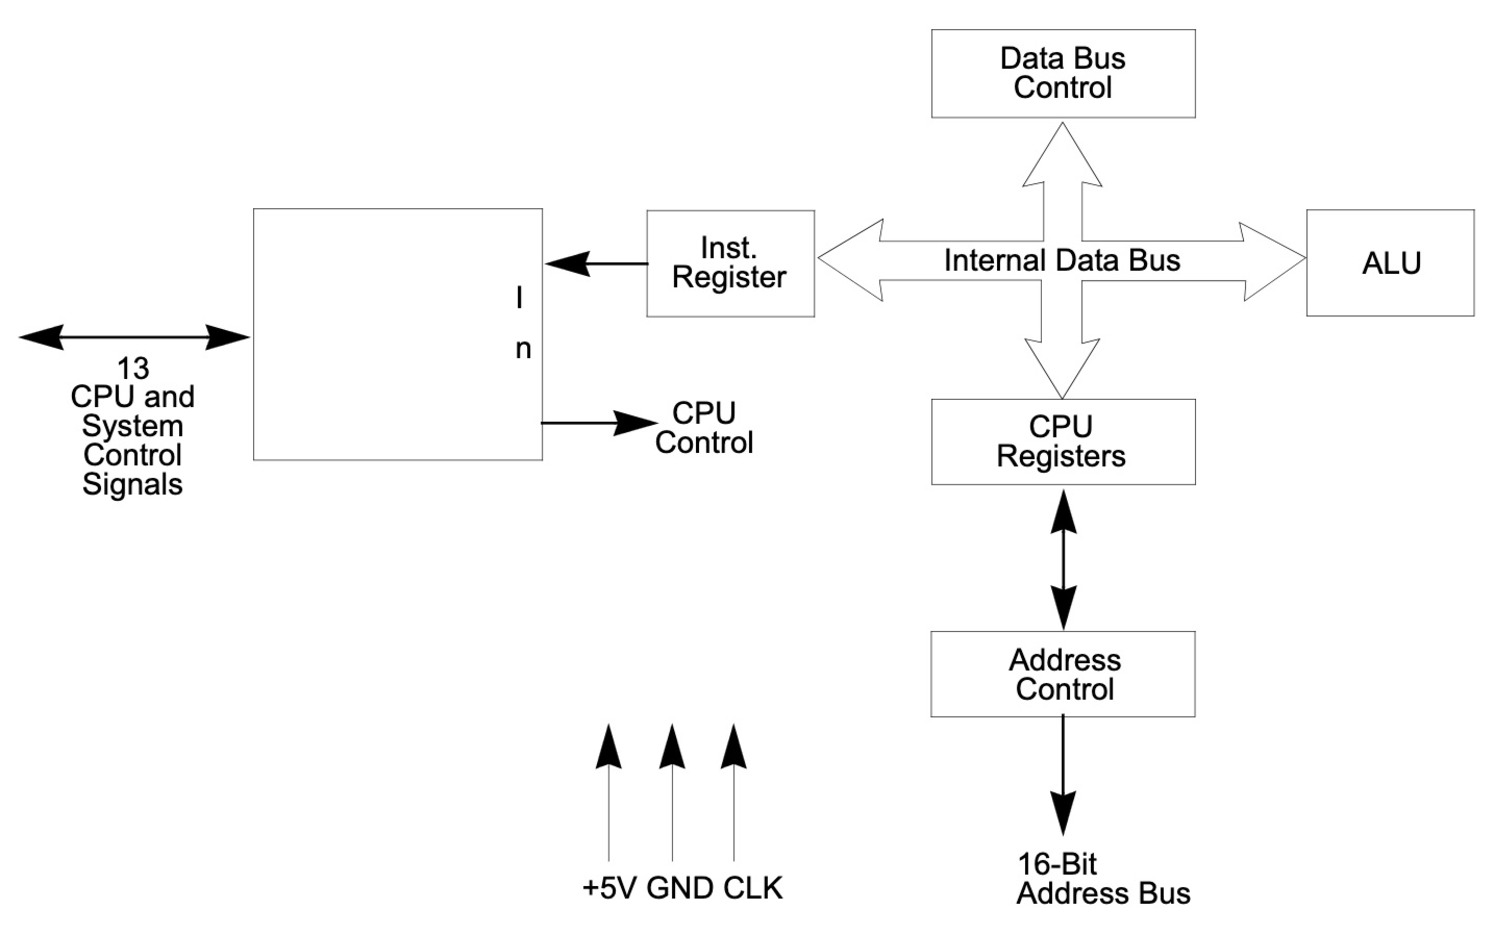
\includegraphics[width=0.7\textwidth]{z80cpuusermanual_pic1}
        \end{center}
        \caption{Diagram notranje arhitekture in glavnih elementov procesorja
        Z80 ~\cite{z80cpuusermanual}.}
        \label{z80cpuusermanual_pic1}
    \end{figure}

    Glavni notranji elementi procesorja so videni na sliki
    \ref{z80cpuusermanual_pic1}. Vsak sistem s procesorjem Z80 mora vsebovati določene
    zunanje strojne elemente, kot so vir napajanja +5V, oscilator, pomnilniške naprave
    (RAM, ROM ali PROM) in vhodno-izhodna vezja, katerih signali so časovno usklajeni
    s procesorjem za nadzor pomnilnika ali perifernih vezij. ~\cite{z80cpuusermanual}

    \section{Registri in zastavice}

    \subsection{Razporeditev registrov, njihove velikosti in pomen}

    Večina operacij Z80 je 8-bitnih, torej dela z vrednostmi med \texttt{0x00}
    in \texttt{0xFF}, kar lahko predstavlja bodisi nepredznačen obseg vrednosti
    od 0 do 255, bodisi predznačen obseg vrednosti od -128 do 127 ~\cite{strojnijezikzaprocesorz80}.

    Nekatere operacije pa so 16-bitne, torej CPE dela z vrednostmi med \texttt{0x0000}
    in \texttt{0xFFFF}, kar lahko predstavlja bodisi nepredznačen obseg vrednosti
    od 0 do 65535, bodisi predznačen obseg vrednosti od -32768 do 32767. 16-bitna
    števila največkrat potrebujemo za naslavljanje pomnilniških celic ~\cite{strojnijezikzaprocesorz80}.

    Posebnost so vrednosti števil v obliki plavajoče vejice, ki zavzemajo kar 5 zlogov
    (prvi zlog vsebuje $128+n$, ostali 4 zlogi vsebujejo mantiso z vrednostjo $[\frac{1
    }{2}, 1)$). Ker 5-zložnih vrednosti ne moremo shraniti v posamezen register ali
    registrski par, za njihovo shranjevanje uporabljamo bodisi celoten
    registrski petorček AFBCDE bodisi računski sklad v pomnilniku. Vendar pa tak tip
    podatka ni specifičen za procesor Z80, temveč za podprograme ROMa
    računalnika ZX Spectrum ~\cite{strojnijezikzaprocesorz80}.

    Procesor Z80 vsebuje 208 bitov bralno-pisalnega pomnilnika, implementiranega
    kot statični RAM, ki predstavlja 18 8-bitnih registrov in 4 16-bitne registre
    ~\cite{z80cpuusermanual}.

    Ti notranji registri se delijo na dva registrska nabora, od katerih vsak vsebuje
    6 splošnonamenskih registrov (registri B, C, D, H in L), akumulator (register
    A) in register zastavic (register F), ter 6 posebnonamenskih registrov, ki so
    16-bitni programski števec (register PC), 16-bitni kazalec sklada (register SP),
    16-bitna indeksna registra IX in IY, osvežitveni register R in register
    naslova strani prekinitev I. Razporeditev notranjih registrov je videna na sliki
    \ref{z80cpuusermanual_pic2} ~\cite{strojnijezikzaprocesorz80} ~\cite{z80cpuusermanual}.

    Pri tem lahko splošnonamenske 8-bitne registre uporabljamo posamično, ali pa
    pare 8-bitnih registrov združimo v 16-bitne registrske pare BC, DE in HL ~\cite{strojnijezikzaprocesorz80}
    ~\cite{z80cpuusermanual}.

    Med uporabo osnovnega in zamenljivega registrskega nabora (katerega imena
    registrov označujemo z apostrofom ob imenih) se lahko preklaplja. Ta
    značilnost procesorja Z80 je posebej potrebna v sistemih, ki zahtevajo hiter odziv
    na prekinitve. Ob pričetku obdelave prekinitev ali izvajanja podprograma je
    potrebno star izvajalni kontekst (vrednosti registrov) shraniti do obnovitve
    pred vrnitvijo iz podprograma. Zamenljiva registrska nabora tako omogočata mnogo
    hitrejšo menjavo konteksta napram hrambi in obnavljanju vrednosti vseh registrov
    v pomnilniku ~\cite{strojnijezikzaprocesorz80} ~\cite{z80cpuusermanual}.

    \begin{figure}[htb]
        \begin{center}
            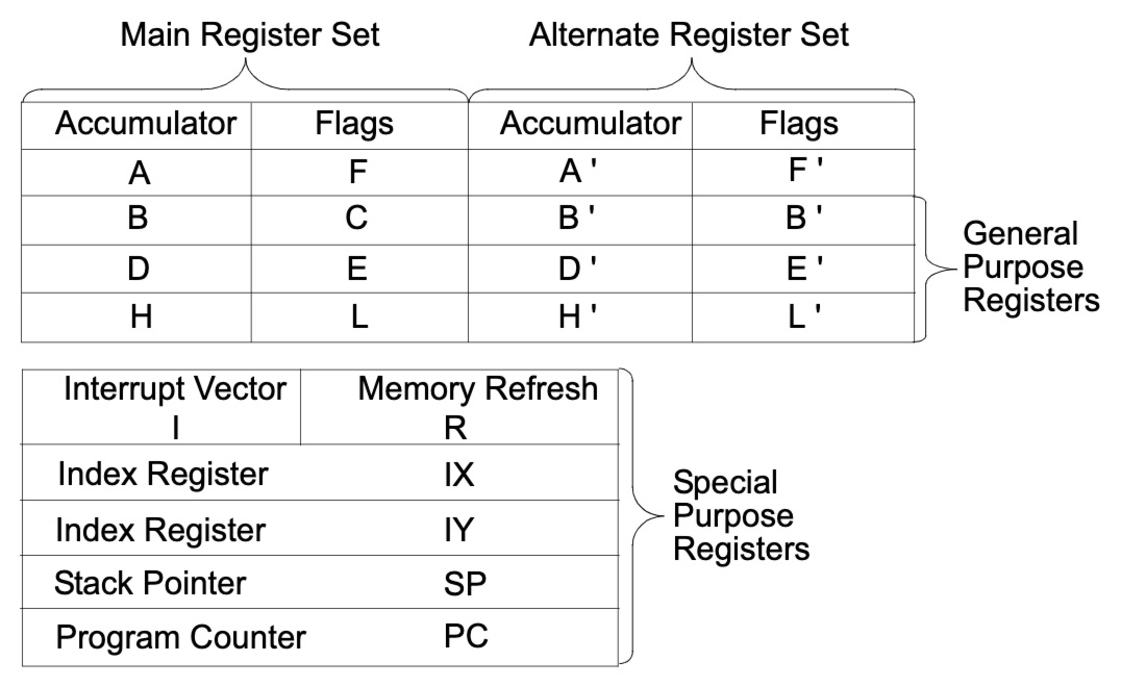
\includegraphics[width=0.7\textwidth]{z80cpuusermanual_pic2}
        \end{center}
        \caption{Diagram notranjih registrov procesorja Z80
        \cite{z80cpuusermanual}.}
        \label{z80cpuusermanual_pic2}
    \end{figure}

    Akumulator oz. register A velja za edini register, kjer procesor lahko
    opravlja 8-bitne aritmetično-logične operacije. Pri njihovem izvajanju register
    zastavic F v splošnem hrani posebne pogoje izvedenih operacij ali značilnosti
    dobljenega rezultata ~\cite{strojnijezikzaprocesorz80} ~\cite{z80cpuusermanual}.

    Register naslova strani prekinitev (I) hrani višji zlog naslova prekinitveno-servisnega
    programa, ki se dopolnejo z nižjim zlogom naslova, ki jih zagotovi zunanja naprava,
    ki je sprožila prekinitev. Procesor Z80 namreč deluje v načinu, v katerem je
    mogoče v odziv na prekinitev izvesti posredni klic na PSP na poljubnem mestu
    v pomnilniku ~\cite{z80cpuusermanual}.

    Register osveževanja pomnilnika (R) hrani 7-bitni števec osveževanja pomnilnika,
    ki se samodejno poveča po vsakem pridobljenem ukazu, osmi bit se uporablja le
    pri ukazu \texttt{LD R, A}. To omogoča enostavno uporabo dinamičnih in statičnih
    pomnilnikov brez upočasnjevanja delovanja CPE (osveževanje se dogaja med
    dekodiranjem prej pridobljenega ukaza) ~\cite{z80cpuusermanual}.

    Za 16-bitne registre in registrske pare velja, da je višji zlog shranjen v registru/registrskem
    paru prvi, nižji pa drugi. Pri tem je potrebno opozoriti, da je tak vrstni
    red ravno obraten kot pri hranjenju 16-bitne vrednosti v pomnilniku, kjer prva
    pomnilniška celica vsebuje nižji del vrednosti, druga pa višjega ~\cite{strojnijezikzaprocesorz80}
    ~\cite{z80cpuusermanual}.

    Indeksna registra IX in IY hranita 16-bitni naslov, ki se uporablja v indeksnem
    načinu naslavljanja kot bazni kazalec, iz katerega po prištetju odmika (dodaten
    zlog, predstavljen kot število v dvojiškem komplementu), dobimo končni
    pomnilniški naslov operanda ~\cite{z80cpuusermanual}.

    Programski števec PC hrani naslov trenutnega ukaza, ki se pridobiva iz
    pomnilnika, in se samodejno poveča, ko se njegova vsebina prenese na
    naslovno vodilo. PC se uporablja tudi za klice in vračanje iz podprogramov,
    pri čemer se povratni naslov hrani na skladu v pomnilniku ~\cite{strojnijezikzaprocesorz80}
    ~\cite{z80cpuusermanual}.

    Kazalec sklada SP hrani naslov vrhnje vrednosti na skladu. Sklad,
    organiziran v obliki LIFO, omogoča preprosto izvajanje večstopenjskih prekinitev,
    teoretično neomejeno gnezdenje podprogramov in poenostavitev mnogih vrst
    manipulacije podatkov ~\cite{strojnijezikzaprocesorz80} ~\cite{z80cpuusermanual}.

    \subsection{Zastavice}

    Zastavice, hranjene v registrih F in F', predstavljajo informacijo o stanju
    bodisi vsebine registra A, ali o ravnokar opravljeni računski operaciji.
    Kljub temu, da ima register F možnost shranjevanja 8 bitov, za dokumentirane
    zastavice uporablja le 6 bitov (bita 3 in 5 se ne uporabljata) ~\cite{strojnijezikzaprocesorz80}
    ~\cite{z80cpuusermanual}:

    \begin{itemize}
        \item zastavica znaka S (angl. Sign flag) na bitu 7 je dvignjena, ko je rezultat
            operacije negativen,

        \item ničelna zastavico Z (angl. Zero flag) na bitu 6 je dvignjena, ko je
            rezultat operacije enak nič,

        \item zastavica polprenosa H (angl. Half carry flag) na bitu 4 je
            dvignjena, ko se je v zadnji operaciji spremenil 5. bit registra,

        \item zastavica parnosti/prepolnjenja P/V (angl. Parity/oVerflow flag)
            na bitu 2 je dvignjena, ko je v rezultatu operacije parno število bitov
            ali ko se je spremenil najvišji bit registra (kar pomeni možnost
            preliva),

        \item zastavica odštevanja N (angl. subtract flag) na bitu 1 je
            dvignjena, ko je zadnja operacija bila odštevanje,

        \item zastavica prenosa C (angl. Carry flag) na bitu 0 je dvignjena, ko se
            je v zadnji operaciji zgodil prenos.
    \end{itemize}

    Zastavice omogočajo vejanje programa prek pogojnih skokov z možnimi pogoji ~\cite{strojnijezikzaprocesorz80}:

    \begin{itemize}
        \item Z (angl. Zero) ob dvignjeni ničelni zastavici,

        \item NZ (angl. Not Zero) ob spuščeni ničelni zastavici,

        \item C (angl. Carry) ob dvignjeni zastavici prenosa,

        \item NC (angl. Not Carry) ob spuščeni zastavici prenosa,

        \item M (angl. Minus) ob dvignjeni zastavici znaka,

        \item P (angl. Positive) ob spuščeni zastavici znaka,

        \item PE (angl. Parity Even) ob dvignjeni zastavici parnosti,

        \item PO (angl. Parity Odd) ob spuščeni zastavici parnosti.
    \end{itemize}

    \subsection{Nedokumentirane zastavice}

    Uradna dokumentacija procesorja Z80 bita 5 in 3 registrov zastavic F in F',
    ki ju bomo označevali kot YF in XF, pogosto obravnava kot neuporabljena,
    vendar ju dejanski procesor vseeno nastavlja in uporablja. Ti zastavici nista
    pogojni zastavici v enakem smislu kot ničelna zastavica Z ali zastavica prenosa
    C, saj Z80 nima pogojnih skokov, klicev ali vrnitev, ki bi neposredno
    preverjali YF ali XF. Zaradi tega se zdita bita za običajno programiranje nepomembna,
    pri emulaciji pa sta pomembna za programe, ki uporabljajo stranske učinke ukazov.
    Zato ju emulator, ki želi natančno posnemati procesor, kljub pomanjkljivi
    uradni dokumentaciji ne sme obravnavati kot neuporabljena ~\cite{theundocumentedz80documented}.

    Pri običajnih aritmetično-logičnih ukazih z 8-bitnim rezultatom se YF in XF praviloma
    nastavita iz bitov 5 in 3 tega rezultata. Pri ukazih primerjave se rezultat
    ne shrani v akumulator, zato se YF in XF nastavita iz bitov 5 in 3 primerjanega
    operanda. Pri 16-bitni aritmetiki se YF in XF nastavita tako, kot da bi ju določila
    operacija nad višjima zlogoma operandov. Pri ukazih preverjanja stanja
    posameznega bita se YF nastavi, kadar ukaz preverja bit 5 in je ta bit postavljen,
    XF pa kadar preverja bit 3 in je ta bit postavljen. A to ne velja pri indeksnem
    naslavljanju, kjer se YF in XF nastavita iz bitov 5 in 3 višjega zloga
    efektivnega naslova indeksiranega naslavljanja, ter pri ukazu \texttt{BIT n,(HL)},
    kjer se YF in XF nastavita iz vrednosti nedokumentiranega notranjega registra,
    povezanega z nekaterimi predhodnimi 16-bitnimi aritmetičnimi ukazi ter
    uporabljenimi efektivnimi naslovi. Pri bločnih ukazih prenosov in primerjav se
    YF in XF nastavita iz vmesnih vrednosti prenosov ali izračunov primerjav.
    Pri bločnih vhodno-izhodnih ukazih se po prenosu zloga najprej zmanjša
    register B, nato pa se YF nastavi iz bita 5 nove vrednosti registra B, XF pa
    iz njenega bita 3 ~\cite{theundocumentedz80documented}.

    \section{Ukazi}
    ZX Spectrum omogoča uporabo visokonivojskega jezika BASIC. Jezik je bil leta
    1964 razvit na Dartmouth College v New Hampshiru, in je bil v svojem času zelo
    razširjen na osebnih računalnikih. Ima več različic, med katerimi obstajajo manjše
    razlike, kot na primer zahteva po zapisu ukazne besede LET pri dodeljevanju
    vrednosti spremenljivkam, kar v mnogih drugih različicah jezika BASIC lahko opustimo.
    A različica BASICa za ZX Spectrum vseeno ni daleč od (neobstoječega standarda)
    jezika BASIC, zato ne bi smeli imeti preveč težav pri prilagajanju katerega koli
    BASIC programa za delovanje na ZX Spectrum ~\cite{zxspectrumintroduction}.

    Za programiranje na Spectrumu lahko uporabljamo tudi strojni jezik, ki v večini
    primerov omogoča hitrejše izvajanje, učinkovitejšo izrabo pomnilnika, krajše programe
    (za hrambo v pomnilniku omejene velikosti) ter neodvisnost od nadzornega programa,
    ki je potreben za izvajanje programov v BASICu. A prinaša tudi nekatere slabosti,
    kot so slabša berljivost programov, omejenost na izvajanje programa v sistemih
    z istim procesorjem, ter nasploh daljši programi (za hrambo v pomnilniku) ~\cite{strojnijezikzaprocesorz80}.

    Berljivost strojnega programa lahko izboljšamo s pisanjem v zbirnem jeziku,
    ki predstavlja preslikavo strojnega jezika v ljudem razumljivejšo obliko, v kateri
    vsak zbirni ukaz ustreza enemu strojnemu ukazu (in obratno). Zbirni jezik je
    tako razumljivejši ljudem, a ga moramo pred izvajanjem prevesti v zaporedje zlogov
    strojnega koda, bodisi ročno, bodisi z uporabo zbirnika. Najbolj razširjen
    zbirnik za uporabo v Spectrumu je bil program GENS ~\cite{zxspectrumbasicprogramming}
    ~\cite{strojnijezikzaprocesorz80}.

    \subsection{Število ukazov in sklopi, njihove dolžine}

    Procesor Z80 lahko izvaja 158 različnih (dokumentiranih) ukazov, vključno z
    vsemi 78 ukazi procesorja 8080A ~\cite{z80cpuusermanual}.

    Vsak ukaz je sestavljen iz zaporedja osnovnih strojnih M-stanj, ta pa so
    sinhrona s časovnimi T-stanji (angl. Transition state), ki predstavljajo čas
    ene urine periode kremenčevega kristala v CPE. Pri frekvenci 3,5 MHz procesorja
    Z80 eno stanje T traja približno 0,2857 mikrosekunde in predstavlja osnovno merilo
    hitrosti operacij ~\cite{strojnijezikzaprocesorz80}.

    Ukaze delimo na več skupin ~\cite{z80cpuusermanual}:
    \begin{itemize}
        \item ukaze nalaganja in izmenjav, ki premikajo podatke med izvorno in
            ciljno lokacijo, bodisi med posameznimi registri ali registri in pomnilnikom,

        \item aritmetične in logične ukaze, ki jih procesor izvaja nad podatki v
            akumulatorju in drugih splošnonamenskih registrih ali pomnilniških
            lokacijah. Rezultat dane operacije se razen v par izjemah shrani v akumulator,
            glede na rezultat operacije pa se nastavijo tudi ustrezne zastavice
            v registru zastavic,

        \item ukaze rotacije in zamikov, ki omogočajo levo ali desno, aritmetično
            ali logično, rotacijo ali zamik vrednosti poljubnega registra ali
            pomnilniške lokacije z ali brez prenosa,

        \item ukaze manipulacije bitov, ki omogočajo nastavitev, ponastavitev ali
            preveritev vrednosti poljubnega bita vrednosti v akumulatorju,
            drugem splošnonamenskem registru ali pomnilniški lokaciji,

        \item ukaze skokov, klicev in vrnitev, ki se uporabljajo za skoke med več
            lokacijami v programu. Edinstvena vrsta klicev so ukazi skupine
            ponovnih zagonov, ki lahko kot nov naslov izvajanja določi le enega od
            8 ločenih naslovov, ki se nahajajo na prvi strani pomnilnika,

        \item ukaze prenosov in iskanja blokov, ki se uporabljajo za prenos
            celih blokov podatkov iz enega mesta pomnilnika na drugo oziroma
            iskanje poljubnega 8-bitnega znaka v bloku podatkov v pomnilniku. Ob dosegu
            konca definiranega bloka ali najdenega znaka se ukaz samodejno prekine,
            prav tako se lahko izvajanje takega ukaza kadarkoli prekine in
            kasneje nadaljuje, kar omogoča vmesno uporabo procesorja za druge operacije.
            Ukazi te skupine pridejo prav pri obdelavi velikih nizov podatkov,

        \item ukaze vhoda in izhoda, ki omogočajo prenose podatkov (posameznih ali
            blokov) med pomnilniškimi lokacijami ali splošnimi registri
            procesorja in zunanjimi V/I napravami,

        \item nadzorni oziroma kontrolni ukazi, ki omogočajo upravljanje
            različnih načinov delovanja procesorja, med drugim omogočanje in onemogočanje
            prekinitev, nastavljanje načina odziva na prekinitve, itd.
    \end{itemize}

    Podskupina ukazov ponovnih zagonov RST (angl. ReSTart) opravlja isto nalogo
    kot brezpogojni klici, le da lahko z njimi kličemo le 8 naslovov v začetku ROMa
    ~\cite{strojnijezikzaprocesorz80}:
    \begin{itemize}
        \item RST \texttt{0x00} učinkuje kot izklop in ponovnen vklop
            računalnika,

        \item RST \texttt{0x08} služi za prikaz sporočila o napaki BASICa, katere
            8-bitni kod napake sledi ukazu kot operand, ter za uporabljanje
            mikrotračnih enot in omrežja Spectrumov preko vmesnika na zadnji
            strani računalnika,

        \item RST \texttt{0x10} na zaslon izpiše znak, katerega kod je v registru
            A,

        \item RST \texttt{0x18} register A napolni z vrednostjo zloga, katerega naslov
            je v sistemski spremenljivki CH-ADD,

        \item RST \texttt{0x20} se uporablja pri tolmačenju programov v BASICu,

        \item RST \texttt{0x28} se uporablja za računanje s plavajočo vejico na
            računskem skladu, zlogi operandi pa določajo operacije, ki se morajo
            izvesti,

        \item RST \texttt{0x30} preuredi delovni pomnilniški prostor tako, da dobimo
            v njem toliko prostih zlogov, kolikor je vrednost registrskega para
            BC,

        \item RST \texttt{0x38} preleti tipkovnico (kontrola pritisnjenih tipk)
            in poveča števec časa.
    \end{itemize}

    *Str. 132-133 - kodi operacij za ukaz RST 28 in tabele podprogramov* ~\cite{strojnijezikzaprocesorz80}

    \subsection{Tipi naslavljanj}

    Naslavljanje se nanaša na način definicije naslova podatkov v registrih, pomnilniku
    ali V/I vratih, ki se bodo uporabili pri izvedbi določenega ukaza ~\cite{z80cpuusermanual}.

    Registrsko naslavljanje (oblike \texttt{LD r, r}) določi enega ali več
    registrov, ki se uporabijo za dano operacijo ~\cite{strojnijezikzaprocesorz80}
    ~\cite{z80cpuusermanual}.

    Sprotno ali takojšnje naslavljanje (oblike \texttt{LD r, n}) v zlogu, ki sledi
    št. strojnega ukaza, vsebuje 8-bitno vrednost operanda ~\cite{strojnijezikzaprocesorz80}
    ~\cite{z80cpuusermanual}.

    Razširjeno takojšnje naslavljanje (oblike \texttt{LD rr, nn}) v zlogih, ki sledita
    št. strojnega ukaza, vsebuje 16-bitno vrednost operanda ~\cite{z80cpuusermanual}.

    Zunanje ali razširjeno naslavljanje (oblik \texttt{LD A, (nn)} in \texttt{LD
    (nn), A)}) v zlogih, ki sledita št. strojnega ukaza, vsebuje pomnilniški naslov
    operanda, kar omogoča prenašanje vrednosti iz registra v pomnilniško celico
    in obratno ter skok ali prenos podatkov med poljubnima pomnilniškima
    lokacijama ~\cite{strojnijezikzaprocesorz80} ~\cite{z80cpuusermanual}.

    Registrsko posredno naslavljanje (oblik \texttt{LD r, (rr)} in \texttt{LD (rr),
    r}) določi registrski par, katerega vrednost predstavlja pomnilniški naslov operanda
    ~\cite{strojnijezikzaprocesorz80} ~\cite{z80cpuusermanual}.

    Relativno naslavljanje v zlogu, ki sledi št. strojnega ukaza, vsebuje odmik
    v obliki dvojiškega komplementa, ki se prišteje vrednosti registra PC za določitev
    pomnilniške lokacije operanda. To poleg prenosljivosti programa omogoča tudi
    skoke na bližnje pomnilniške lokacije z le dvozložnim ukazom ~\cite{z80cpuusermanual}.

    Indeksno naslavljanje (oblik \texttt{LD r, (IX+dis)} in \texttt{LD (IX+dis), r})
    je le oblika registerskega posrednega naslavljanja z dodanim odmikom. V
    zlogu, ki sledi št. strojnega ukaza, vsebuje odmik v predstavitvi dvojiškega komplementa,
    ki se prišteje vrednosti izbranega indeksnega registra za določitev
    pomnilniške lokacije operanda. To poleg prenosljivosti programa omogoča tudi poenostavitev
    dela s tabelami podatkov ~\cite{strojnijezikzaprocesorz80} ~\cite{z80cpuusermanual}.

    Bitno naslavljanje s pomočjo registrskega, registerskega posrednega ali
    indeksnega naslavljanja lahko določi poljubni bit poljubne pomnilniška
    lokacije ali registra za izvedbo bitne operacije ~\cite{z80cpuusermanual}.

    Spremenjeno naslavljanje ničelne strani se nanaša na posebne enozložne ukaze RST
    za skok na poljubno od 8 lokacij v strani 0 pomnilnika, kjer se nahajajo
    pogosto uporabljeni podprogrami ROMa ~\cite{z80cpuusermanual}.

    Implicitno naslavljanje se uporablja pri mnogih ukazih, ki implicitno
    določijo registre z operandi, potrebnimi za dano operacijo (npr. rezultat aritmetičnih
    operacij se implicitno shrani v akumulator) ~\cite{z80cpuusermanual}.

    Ker mnoge operacije zahtevajo več kot en operand, se lahko hkrati uporabi
    tudi več tipov naslavljanj ~\cite{z80cpuusermanual}.

    \subsection{Nedokumentirani ukazi}

    Poleg uradno navedenega nabora ukazov ima Z80 tudi množico operacijskih kod, ki
    so v uradni dokumentaciji izpuščene ali označene kot neuporabljene. Na
    pravem procesorju te operacijske kode kljub temu lahko izvedejo nove ali
    podvojene že dokumentirane ukaze. To se zgodi zato, ker procesor tudi pri
    nedokumentiranih kombinacijah bitov uporabi isto dekodirno logiko kot pri
    uradnem naboru ukazov. Predpona določi skupino ukazov, naslednji zlogi pa
    določijo operacijo, register ali način naslavljanja ~\cite{theundocumentedz80documented}.

    Pri predponi \texttt{0xCB} nedokumentirane kode od \texttt{0xCB30} do
    \texttt{0xCB37} med drugim definirajo ukaze logičnih pomikov v levo \texttt{SLL}.
    Pri predponi \texttt{0xDD} se uporabe registra HL v ukazih praviloma
    nadomestijo z IX, pri predponi \texttt{0xFD} pa z IY, vključno z dostopi do posameznih
    polovic oziroma zlogov indeksnih registrov. Pri predponi \texttt{0xED} nekatere
    kode predstavljajo dvojnike uradnih ukazov, preostale neuporabljene kode pa
    se obnašajo kot zaporedja brez učinka. Posebnost sta ukazni kodi \texttt{0xED70}
    in \texttt{0xED71}, od katerih prva prebere vrednost iz V/I vrat in z njo
    nastavi samo zastavice, druga pa na V/I vrata zapiše vrednost nič. Pri
    štirizložnih skupinah s predponama \texttt{0xDD 0xCB} in \texttt{0xFD 0xCB}
    se bitne operacije izvedejo nad indeksirano pomnilniško lokacijo, pri delu ukazov
    pa zadnji zlog določi še dodatni ciljni register ~\cite{theundocumentedz80documented}.

    \section{Prekinitve}

    Prekinitve omogočajo prekinitev operacij CPE, izvajanja PSP in vrnitev v
    prvotno stanje izvajanje programa. Prekinitev lahko sproži zunanja naprava ali
    nadzorni program računalnika. Na primer, CPE vsako 1/50 sekunde pogleda stanje
    posebne notranje zastavice IFF1. Če je njena vrednost 1, sproži prekinitev in
    izvrši ukaz RST 38H, s katerim pridobi stanje tipkovnice ~\cite{strojnijezikzaprocesorz80}
    ~\cite{z80cpuusermanual}.

    Ker se zaradi tega delovna hitrost procesorja nekoliko zmanjša, lahko program
    z ukazom DI prekinitve onemogoči in kasneje z ukazom EI nazaj omogoči.
    Program lahko prav tako ukazom HALT prekine izvajanje strojnega programa do
    naslednje prekinitve. Med tem CPE izvaja operacije NOP za namen delovanja osveževanja
    pomnilnika ~\cite{strojnijezikzaprocesorz80} ~\cite{z80cpuusermanual}.

    \subsection{Načini prekinitev in njihovo delovanje}

    Z80 CPE podpira 2 vrsti prekinitev:

    Maksabilne prekinitve INT, ki jih je mogoče programsko onemogočiti, z
    nastavljanjem vrednosti IFF1 prek ukazov EI in DI, saj se uporablja kot zahteva
    za prekinitev s strani zunanjih naprav. CPE ima poleg notranje zastavice
    IFF1, ki se dejansko uporablja pri izvajanju, še IFF2 kot začasno shrambo
    vrednosti IFF1. Glavna stanja obeh notranjih zastavic in spremembe ob pomembnih
    ukazih so videne v tabeli \ref{z80cpuusermanual_tab2} ~\cite{z80cpuusermanual}.

    \begin{table}[htb]
        \begin{center}
            \begin{tabular}{|p{0.28\textwidth}|c|c|p{0.42\textwidth}|}
                \hline
                \textbf{Dejanje}              & \textbf{IFF1} & \textbf{IFF2} & \textbf{Opombe}                                                          \\
                \hline
                Ponastavitev CPE              & 0             & 0             & Prekinitve so onemogočene.                                               \\
                \hline
                Izvedba ukaza \texttt{DI}     & 0             & 0             & Prekinitve so onemogočene.                                               \\
                \hline
                Izvedba ukaza \texttt{EI}     & 1             & 1             & Prekinitve so omogočene.                                                 \\
                \hline
                Izvedba ukaza \texttt{LD A,I} & *             & *             & Vrednost IFF2 se shrani v zastavico paritete.                            \\
                \hline
                Izvedba ukaza \texttt{LD A,R} & *             & *             & Vrednost IFF2 se shrani v zastavico paritete.                            \\
                \hline
                Sprejem NMI                   & 0             & *             & Prekinitve so onemogočene.                                               \\
                \hline
                Izvedba ukaza \texttt{RETN}   & IFF2          & *             & Dvignjena IFF2 označi konec rutine za obdelavo nemaskabilnih prekinitve. \\
                \hline
            \end{tabular}
        \end{center}
        \caption{Tabela stanj in sprememb stanj IFF1 in IFF2 ~\cite{z80cpuusermanual}.}
        \label{z80cpuusermanual_tab2}
    \end{table}

    CPE je lahko nastavljen v enega izmed 3 možnih načinov obravnavanja maskabilnih
    prekinitev ~\cite{z80cpuusermanual}.

    V načinu 0 lahko prekinitvena naprava na podatkovno vodilo postavi poljuben
    ukaz, ki ga CPE izvede. Ker mora izbran ukaz imeti le 1 zlog, je to pogosto ukaz
    klica PSP. CPE pri izvedbi tega ukaza samodejno doda 2 čakalni periodi, da bi
    zagotovil dovolj časa za izvedbo zunanje verižne povezave za nadzor prioritet
    ~\cite{z80cpuusermanual}.

    V načinu 1 CPE začne izvajati ukaz na pomnilniškem naslovu \texttt{0x0038}.
    Posledično je odziv razen lokacije klica identičen odzivu na nemaskabilne
    prekinitve, ki kliče podprogram na pomnilniškem naslovu \texttt{0x0066}. CPE tudi
    v tem primeru doda 2 čakalni periodi ~\cite{z80cpuusermanual}.

    Način 2 omogoča klic podprograma v uporabniško vzdrževani tabeli 16-bitnih
    začetnih naslovov PSP na poljubnem mestu v pomnilniku. Naslovi PSP v tabeli se
    morajo nahajati na sodih naslovih, ker vsak zavzema 2 zloga. Zgornji zlog 16-bitnega
    naslova PSP določa vrednost registra I, spodnji zlog pa sama prekinitvena
    naprava. Ko prekinitvena naprava zagotovi spodnji del kazalca, CPE samodejno
    potisne PC na sklad, pridobi naslov PSP iz tabele in izvede skok nanj. Ta
    način odziva zahteva 19 čakalnih period ~\cite{z80cpuusermanual}.

    Prekinitve NMI imajo višjo prioriteto kot INT in jih ni mogoče programsko onemogočiti,
    saj se uporablja za predvsem za takojšnje odzive na najpomembnejše signale, ki
    se morajo obravnavati s čim manj zakasnitve. CPE ga zato obravnava že po
    koncu izvajanja trenutnega ukaza. Pri tem se najprej IFF1 onemogoči (in
    njegova prejšnja vrednost shrani v IFF2), kar za čas izvajanja PSP prepreči
    navadne prekinitve, nato se vrednost registra PC shrani na sklad, izvajanje
    pa preusmeri na pomnilniški naslov \texttt{0x0066} ~\cite{z80cpuusermanual}.

    \section{Implementacija v emulatorju}

    Procesor je v emulatorju predstavljen z objektom \texttt{Processor}. Ta ne hrani
    vseh podatkov procesorja neposredno v sebi, ampak povezuje ločene modele
    registrov, pomnilnika, V/I vrat in časovnika. Časovni model je implementiran v
    objektu \texttt{ULATiming}, ki hrani skupno število izvedenih T-stanj,
    trenutno pozicijo znotraj slikovnega okvira in števec prikazanih okvirjev. Emulator
    privzeto uporablja frekvenco procesorja 3,5 MHz in dolžino okvirja 69888 T-stanj,
    kar ustreza modelu računalnika 48K z evropskim video standardom. V objektu \texttt{Processor}
    so shranjena predvsem stanja, ki vodijo izvajanje, kot so omogočenost
    maskabilnih prekinitev \texttt{IFF1} in \texttt{IFF2}, trenutni prekinitveni način,
    stanje \texttt{HALT}, prekinitvene točke in števec izvedenih ukazov.

    Registri so zbrani v objektu \texttt{Registers}. Ta vsebuje glavni in
    zamenljiv registrski nabor ter posebne registre \texttt{I}, \texttt{R},
    indeksna registra \texttt{IX} in \texttt{IY}, \texttt{SP}, \texttt{PC} in
    nedokumentirani notranji register \texttt{MEMPTR}. Zastavice niso ločen
    podatkovni tip, ampak posamezni biti v registru \texttt{F}. Dostop do njih je
    zato implementiran z metodami za branje in nastavljanje posameznih bitov.

    Posamezen strojni ukaz je predstavljen z vmesnikom \texttt{Instruction}. Ukaz
    pozna naslov, zloge, iz katerih je bil dekodiran, število T-stanj in metodo
    \texttt{execute}, ki izvede vse potrebne spremembe na stanju sistema ob
    izvedbi. Opis ukaza je ločen od njegove izvedbe z vmesnikom \texttt{InstructionDefinition}.
    Definicija vsebuje bitni vzorec ukaznega zloga oziroma zaporedja zlogov in metodo
    za dekodiranje operandov.

    Bitni vzorci so opisani z razredom \texttt{BitPattern}. V njem so fiksni biti
    zapisani kot ničle in enice, ostali znaki pa predstavljajo zajeta polja, na primer
    kodo registra, pogoj skoka, neposredni zlog ali 16-bitni operand. Dekodirnik
    v objektu \texttt{Instructions} iz pomnilnika prebere toliko zlogov, kot jih
    zahteva posamezen vzorec, prebrano vrednost primerja z registriranimi vzorci in
    ob ujemanju ustvari konkreten objekt ukaza.

    Posebna obravnava je potrebna pri predponah kodov ukazov. Predponi \texttt{DD}
    in \texttt{FD} pomenita, da se nekateri dostopi do \texttt{HL}, \texttt{H}
    in \texttt{L} začasno preusmerijo na \texttt{IX} oziroma \texttt{IY}. To je
    v emulatorju izvedeno z začasnim načinom indeksne predpone v objektu \texttt{Registers}.
    Dekodirnik zna obravnavati tudi kombinacije s predponama \texttt{CB} in \texttt{ED}
    ter več zaporednih indeksnih predpon. Tak ukaz se ovije v pomožni objekt, ki
    ohrani izvorne zloge, prišteje dodatna T-stanja za predpone in nastavi pravilen
    način dostopa do indeksnih registrov le za čas izvedbe takega ukaza.

    Izvajanje enega koraka (naslednjega ukaza) se začne z branjem trenutnega programskega
    števca \texttt{PC}. Če je na tem naslovu nastavljena prekinitvena točka, se
    neprekinjen tek ustavi. Nato ima prednost morebitna nemaskabilna prekinitev.
    Če je ni, se preverijo še pogoji za hitro nalaganje kasetnih podatkov. Šele
    nato se ukaz dekodira iz pomnilnika, števec osveževanja \texttt{R} se poveča
    za število dejansko prebranih ukaznih zlogov, programski števec pa se pomakne
    za dolžino ukaza.

    Po predpripravi ukaza se izvede metoda \texttt{execute}. Ta lahko spremeni registre,
    zapisuje v pomnilnik, bere ali piše V/I vrata. Po izvedbi se poveča števec
    izvedenih ukazov za namene razhroščevalnika, časovniku ULA pa se prišteje število
    T-stanj ukaza. Ko število T-stanj preseže dolžino okvirja, časovnik poveča števec
    okvirjev, označi čakajočo prekinitev in o tem obvesti dele uporabniškega
    vmesnika, ki so vezani na osveževanje slike. Pogoji za izvedbo maskabilne
    prekinitve se preverjajo ob koncu izvajanja trenutnega ukaza, zato časovnik povezuje
    hitrost izvajanja, periodične prekinitve in osveževanje zaslonskega prikaza.

    Pri vseh maskabilnih prekinitvah se trenutna vrednost registra \texttt{PC} najprej
    zapiše na sklad, nato se onemogočita \texttt{IFF1} in \texttt{IFF2}. Maskabilna
    prekinitev ponastavi vrednost le \texttt{IFF1}, na sklad shrani vrednost registra
    \texttt{PC} in nadaljuje izvajanje na naslovu \texttt{0x0066}. Ukaza \texttt{EI}
    in \texttt{DI} nastavita še notranjo zastavico, zaradi katere se maskabilna prekinitev
    ne obdela takoj za njima.

    Ukaz \texttt{HALT} je izveden tako, da programski števec vrne na naslov ukaza
    \texttt{HALT} in nastavi stanje zaustavitve. Dokler ne pride do prekinitve,
    se zato ob vsakem koraku znova izvaja isti ukaz, v tem primeru ukaz \texttt{NOP}.
    Ob prekinitvi se stanje \texttt{HALT} zaključi, na sklad pa se zapiše naslov naslednjega
    ukaza, kot pri pravem procesorju.

    Poleg izvajanja ukazov po korakih emulator podpira tudi neprekinjen tek. V tem
    načinu delovanja procesor ponavlja izvajanje ukazov, dokler uporabnik
    emulatorja ne zaustavi. V načinu delovanja emulatorja ob standardni hitrosti primerja
    število izvedenih T-stanj z realnim časom izvajanja in po potrebi počaka z izvajanjem
    nadaljnjega ukaza, da se izvajanje približa frekvenci 3,5 MHz. V načinu delovanja
    emulatorja ob najvišji možni hitrosti tega čakanja ni, zato emulator izvaja
    ukaze tako hitro, kot dopušča gostiteljski sistem.

    Pravilnost implementacije ukazov je bila preverjana tudi s programoma \texttt{zexdoc}
    in \texttt{zexall}, različicama preizkuševalnika ukazov Z80, prilagojenima za
    ZX Spectrum. \texttt{zexdoc} preverja dokumentirane zastavice, registre in
    pomnilnik, \texttt{zexall} pa poleg tega preverja tudi nedokumentirani
    zastavici XF in YF. Programa izvajata skupine ukazov z različnimi začetnimi stanji,
    iz končnega stanja izračunata kontrolno vsoto CRC in jo primerjata z
    referenčno vrednostjo, pridobljeno na pravem procesorju Z80. Preizkus ne
    pove, katera podrobnost ukaza je napačna, temveč samo, da se rezultat razlikuje
    od referenčnega izvajanja ~\cite{z80exerciseravery} ~\cite{spectrumz80exerciser}.

    \chapter{ULA}
    \label{ula}

    Procesorja pri branju in pisanju iz pomnilniških lokacij ne zanima s katerim delom
    pomnilnika dela, pa naj bo to ROM ali RAM. Ve le, da obstaja 65536
    pomnilniških celic, v katerih lahko obdeluje shranjene podatke. Na popolnoma
    enak način dela tudi s 65536 V/I naslovi, od katerih je odvisno delovanje zunanjih
    naprav, kot so tipkovnica, zvočnik, kasetofon prek vtičnic EAR in MIC, tiskalnik
    in drugi robni vmesniki in naprave pa prek robnega priključka, dostopni na
    zadnji strani računalnika ~\cite{zxspectrumbasicprogramming} ~\cite{strojnijezikzaprocesorz80}.

    V/I naslovi so pri procesorju Z80 sestavljeni iz 16 bitov (A15, A14, ..., A1,
    A0), vendar imajo posamezni biti pri Spectrumu različen pomen. Nižji zlog
    naslova označuje ena izmed 256 možnih V/I vrat, zato se operacije na različnih
    V/I naslovih lahko nanašajo na isto operacijo ~\cite{zxspectrumbasicprogramming}
    ~\cite{strojnijezikzaprocesorz80}.

    Vrednosti na V/I naslovih, ki prehajajo med V/I vrati in CPE so sestavljena
    sestavljena iz 8 bitov ~\cite{zxspectrumbasicprogramming} ~\cite{strojnijezikzaprocesorz80}.

    Naslov V/I vrat 251 se nanaša na tiskalnik, naslovi vrat 254, 247 in 239 pa
    na dodatne zunanje naprave, med drugim se naslov V/I vrat 254 nanaša na zvočnik
    (D4), MIC vtičnico (D3) in nastavlja barvo obrobe zaslona (D2, D1 in D0) ~\cite{zxspectrumbasicprogramming}.

    \section{Zaslon}
    V času nastanka računalnika ZX Spectrum so se uporabljali UHF televizorji, kateremu
    je računalnik oddajal zaslonski signal na UHF kanalu 36. Pomembna je bila tudi
    različica računalnika, saj so se standardi televizorskih sistemov
    razlikovali po državah in celinah - evropski in britanski televizorji takrat
    prikazovali 50 slik na sekundo, sistemi v ZDA, Kanadi in Japonski pa 60 slik
    na sekundo. Zaradi tega so zanje delali drugačno verzijo računalnika ~\cite{zxspectrumintroduction}.

    \subsection{Razdelitev}
    Televizijski zaslon ima zunanji del, ki se imenuje obroba zaslona, in
    osrednji del, ki ga imenujemo papir oziroma zaslonska slika. Slednja je je
    razdeljena na 768 položajev znakov (prek 24 vrstic in 32 stolpcev), na katerih
    se prikazujejo znaki. Vsak znak je tako predstavljen kot 8x8 kvadrat točk, ki
    ga lahko shranimo v 8 zlogih (vsak za eno vrstico točk), vsaka točka pa z
    enim bitom, ki določa barvo točke - barva papirja če ima pripadajoč bit vrednost
    0, bodisi v barvo črnila z vrednostjo bita 1 ~\cite{zxspectrumintroduction} ~\cite{zxspectrumbasicprogramming}.

    A vrstice točk, ki določajo prikaz znaka, niso shranjene v zaporednih
    pomnilniških celicah, saj snop elektronov v televiziji potuje po posamezni vrstici
    točk cele vrstice znakov, zaradi česar potrebuje za učinkovito delovanje te
    informacije shranjene zaporedno. V pomnilniku so v takem zaporedju vrstic točk
    znakov shranjene najprej vrstice položajev znakov 0 do 7, nato 8 do 15, in nazadnje
    16 do 23 ~\cite{zxspectrumbasicprogramming}.

    *Str. 76 - prikaz delitve zaslona na vrstice in stolpce* ~\cite{zxspectrumbasicprogramming}

    *Str. 114 - Diagram razbiranja naslovov znakov na zaslonu v pomnilniški zaslonski
    datoteki* ~\cite{strojnijezikzaprocesorz80}

    \subsection{Nabor znakov}
    Nabor 256 znakov, ki ga uporablja ZX Spectrum, sestavljajo ~\cite{zxspectrumbasicprogramming}:
    \begin{itemize}
        \item pozamezne znake iz standarda ASCII (razen simbolov £ in ©) ter grafične
            simbole, značilne le za ZX Spectrum, katerih je prvih 16 sistemsko definiranih
            (vidimo jih na sliki \ref{zxspectrumbasicprogramming_pic1}), drugih
            21 pa uporabniško-definiranih

        \item žetoni, ki predstavljajo bodisi kontrolne znake z učinki na
            zunanje naprave, bodisi navodila računalniku v obliki celih besed (npr.
            PRINT, STOP, ipd.)
    \end{itemize}

    \begin{figure}[htb]
        \begin{center}
            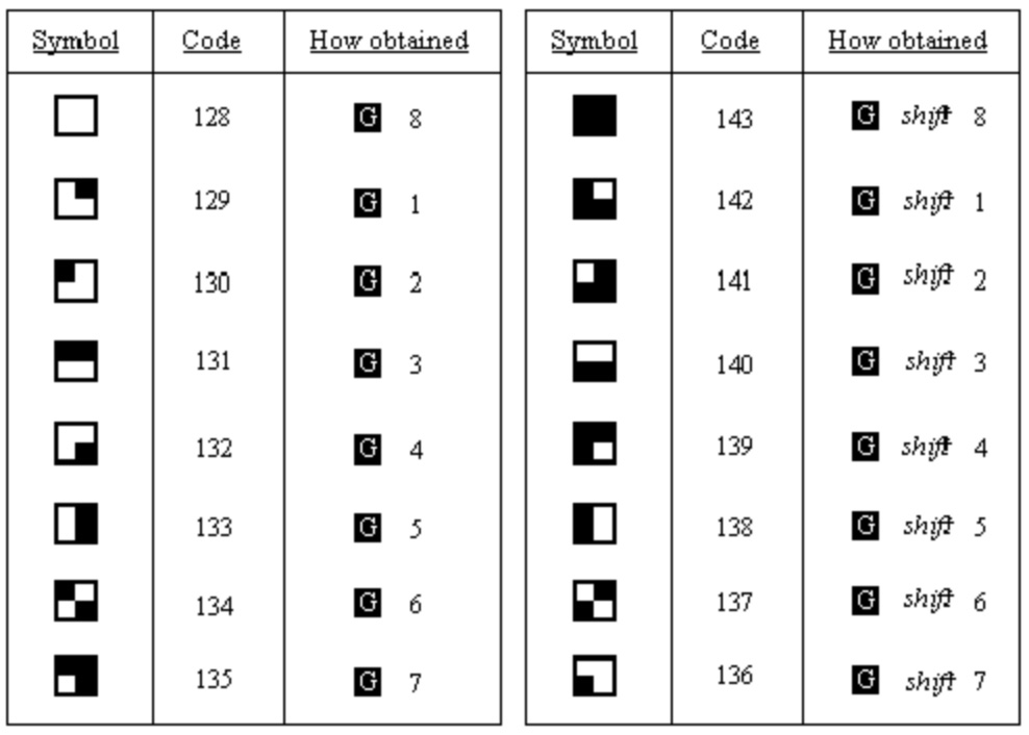
\includegraphics[width=0.7\textwidth]{
                zxspectrumbasicprogramming_pic1
            }
        \end{center}
        \caption{Tabela sistemsko definiranih grafičnih simbolov ~\cite{zxspectrumbasicprogramming}.}
        \label{zxspectrumbasicprogramming_pic1}
    \end{figure}

    V ROMu so med naslovoma 3D00 in 3FFF shranjeni točkovni vzorci vseh znakov
    razen grafičnih simbolov. Naslov posameznega znaka, ki ima kod $x$ (npr.
    znak 'a' ima kod 0x61) izračunamo po formuli $8x+3C00$ ~\cite{strojnijezikzaprocesorz80}.

    \subsection{Atributi znakov}
    Vsak znak ima določene sledeče atribute v enem zlogu ~\cite{zxspectrumintroduction}
    ~\cite{zxspectrumbasicprogramming} ~\cite{strojnijezikzaprocesorz80}:
    \begin{itemize}
        \item bit svetlosti ima dve možni vrednosti: 0 za normalne ali 1 za
            svetlejše barve,

        \item bit utripanja ima dve možni vrednosti: 0 za stalne barve ali 1 za
            utripanje, ki se prikaže kot zaporedno zamenjavanje barve črnila in papirja,

        \item trojica bitov koda barve papirja (privzeto bela),

        \item trojica bitov koda barve črnila (privzeto črna),
    \end{itemize}

    ZX Spectrum lahko na (barvnem) zaslonu prikazuje osem barv, označene s kodi
    od 0 do 7 ~\cite{zxspectrumintroduction} ~\cite{zxspectrumbasicprogramming}:
    \begin{itemize}
        \item 0, ki označuje črno

        \item 1, ki označuje modro

        \item 2, ki označuje rdečo

        \item 3, ki označuje vijolično ali magenta

        \item 4, ki označuje zeleno

        \item 5, ki označuje svetlo modro ali cian

        \item 6, ki označuje rumeno

        \item 7, ki označuje belo
    \end{itemize}

    Čeprav so barve na prvi pogled razporejene v naključnem vrstnem redu, je tak zaradi
    dveh razlogov. Prvi razlog se nanaša na uporabo računanika na črno-belih
    zaslonih, kjer se barve v danem vrstnem redu prikažejo v lestvici odtenkov sivin.
    Drugi razlog se opira na dejstvo, da lahko človeško oko resnično vidi le tri primarne
    barve (modro, rdečo in zeleno), druge barve pa so le njihove mešanice. Tak
    vrstni red barv omogoča "mešanje" barv s seštevanjem kodov primarnih barv. Na
    primer, magenta je pravzaprav mešanica modre in rdeče barve, zato je njen kod
    (3) vsota kodov za modro (1) in rdečo (2) ~\cite{zxspectrumintroduction} ~\cite{zxspectrumbasicprogramming}.

    Kot barvo črnila ali papirja lahko nastavimo tudi vrednosti ~\cite{zxspectrumbasicprogramming}:
    \begin{itemize}
        \item 8, ki označuje "prozorno", pri kateri bo barva ob izpisu znaka ostala
            nespremenjena glede na barvo prejšnjega znaka

        \item 9, ki pomeni "kontrast", pri kateri bo barva nastavljena v kontrastu
            z drugo - bela, če je druga barva temna (črna, modra, rdeča ali magenta)
            ali črna, če je druga barva svetla (zelena, cian, rumena ali bela)
    \end{itemize}

    Enozložna vrednost atributa se nanaša na vseh 64 pik položaja znaka, ne le na
    posamezne pike znaka. Ko znak natisnemo na zaslon, poleg vzorca pik spremenimo
    tudi nastavitve atributov položaja znaka ~\cite{zxspectrumbasicprogramming}.

    \subsection{Implementacija v emulatorju}

    Zaslonski del emulatorja je razdeljen na logiko za razlago pomnilniškega zapisa
    in na prikaz v uporabniškem vmesniku. Objekt \texttt{ULAScreen} vsebuje stalne
    vrednosti za velikost slike, velikost obrobe, začetne in končne naslove zaslonske
    datoteke ter datoteke atributov. V njem je definirana tudi preslikava
    Spectrumovih barv v barve uporabniškega vmesnika ter funkcije za razlago
    bitov enozložne vrednosti atributa.

    Okno zaslona ob periodičnih prekinitvah, ki jih proži ULA za posodobitev izrisa
    zaslonske slike, iz pomnilnika prebere območji zaslonske datoteke in
    datoteke atributov na naslovih \texttt{0x4000}-\texttt{0x57FF} in \texttt{0x5800}-\texttt{0x5AFF}.
    Funkcija za izračun indeksa zloga zaslonske datoteke upošteva ne-linearen razpored
    vrstic, ki ga uporablja ZX Spectrum. Prikaz je narejen z grafično komponento platna
    ogrodja Compose, pri čemer se velikost navidezne točke prilagodi velikosti
    okna, da ostane razmerje slike, uporabljano v zaslonih po standardnih
    televizijah v času nastanka računalnika, nespremenjeno. Tako se izognemo
    nepravilnim proporcijam navideznih točk in posledično popačenju slike.

    \section{Tipkovnica}

    Znaki, ki jih ZX Spectrum prepozna in uporablja, ne vključujejo le posameznih
    znakov, kot so črke, številke in simboli, ampak tudi sestavljene znake, kot so
    ključne besede in imena funkcij ~\cite{zxspectrumbasicprogramming}.

    Tipkovnica Spectruma je na prvi pogled po položaju tipk črk in številk
    podobna tipkovnici navadnega pisalnega stroja, vendar pa ima vsaka tipka Spectruma
    več funkcij. Razporeditev tipk je videna na sliki \ref{softspectrum48_pic1}
    ~\cite{zxspectrumintroduction}.

    \begin{figure}[htb]
        \begin{center}
            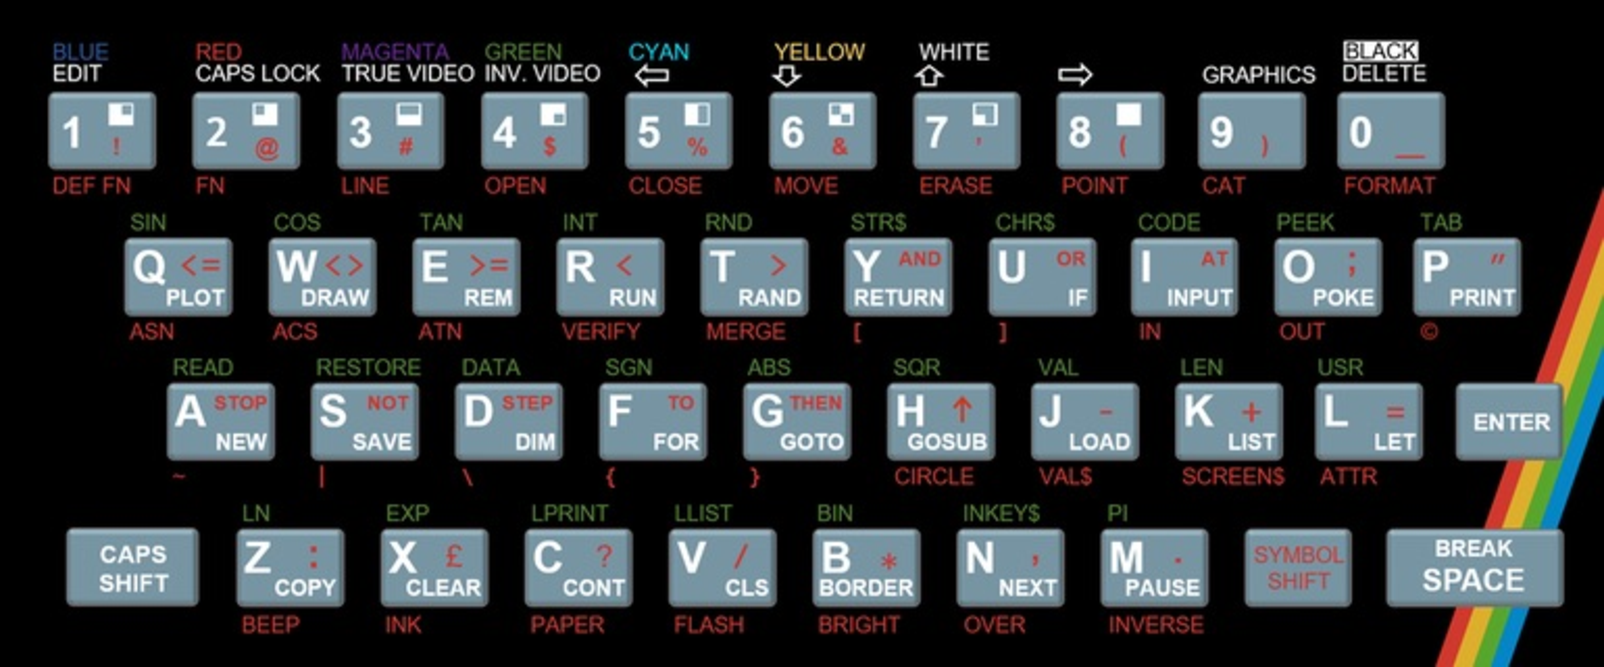
\includegraphics[width=0.7\textwidth]{softspectrum48_pic1}
        \end{center}
        \caption{Shema razporeditve tipk tipkovnice ZX Spectruma ~\cite{softspectrum48}.}
        \label{softspectrum48_pic1}
    \end{figure}

    Da bi lahko z omejenim številom tipk na tipkovnici lahko dostopali do vseh
    znakov in ukazov, imajo nekatere tipke več različnih pomenov, do katerih
    pridemo z uporabo modifikacijskih tipk CAPS SHIFT ali SYMBOL SHIFT ter
    menjavanjem načina delovanja tipkovnice. Povezava med simboli na tipkah in načini
    vnosa je videna na sliki \ref{zxspectrumbasicprogramming_pic2} ~\cite{zxspectrumbasicprogramming}.

    \begin{figure}[htb]
        \begin{center}
            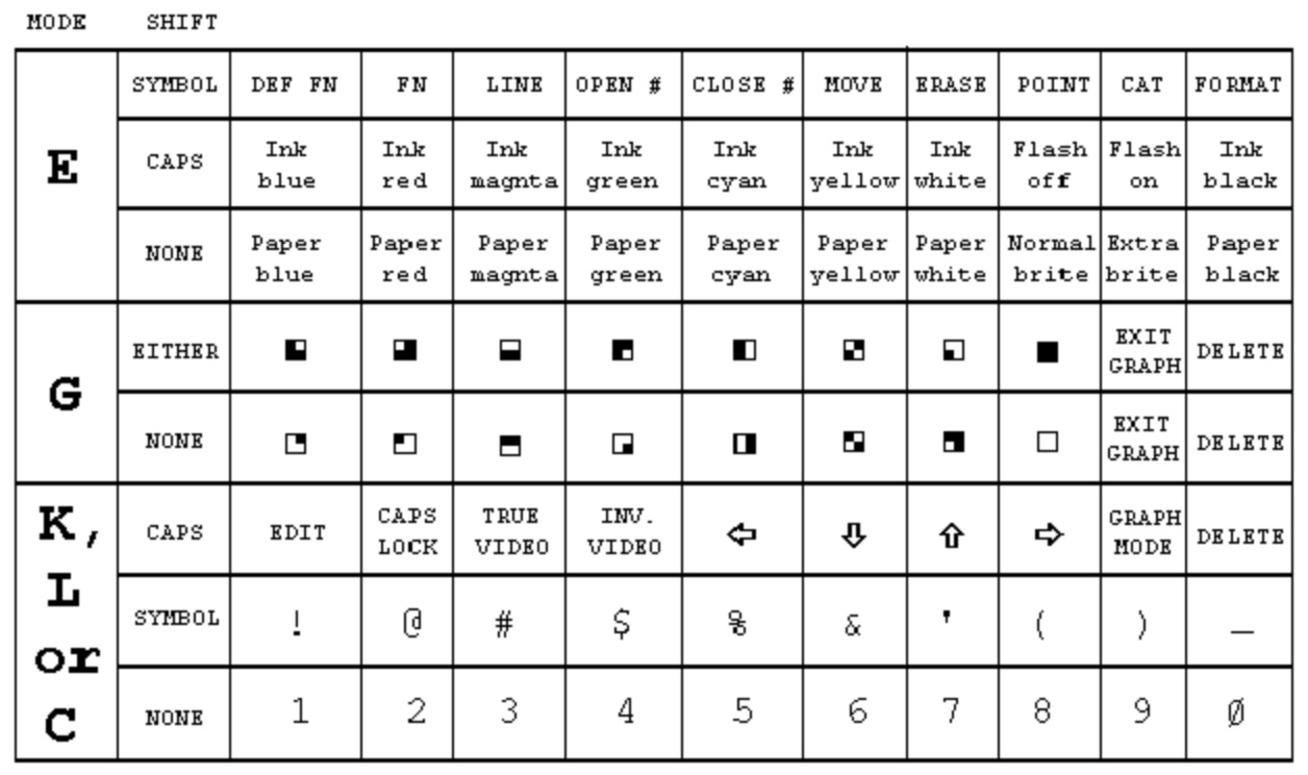
\includegraphics[width=0.7\textwidth]{
                zxspectrumbasicprogramming_pic2
            }
        \end{center}
        \caption{Tabela simbolov in potrebnih pritiskov tipk zanje ~\cite{zxspectrumbasicprogramming}.}
        \label{zxspectrumbasicprogramming_pic2}
    \end{figure}

    \subsection{Načini delovanja}

    Kurzor, predstavljen kot utripajoča črka, hkrati označuje položaj izpisa
    naslednje vnešenega znaka in trenutni način delovanja tipkovnice s črko
    kurzorja ~\cite{zxspectrumintroduction} ~\cite{zxspectrumbasicprogramming}.

    Ko Spectrum prvič vklopite, ta po sporočilu o avtorskih pravicah pričakuje vnos
    ukaza, ki se začne s ključno besedo, katere so natisnjene pod glavnimi simboli
    na tipkah. Za razliko od večine drugih računalnikov Spectrum omogoča vnos
    ključnih besed z enim samim pritiskom na tipko. Kurzor s simbolom K (angl. Keyword)
    predstavlja ta način delovanja za vnos ključnih besed, ki samodejno nadomesti
    način L, ko naprava pričakuje vnos ukaza ali programske vrstice, kar je odvisno
    od pozicije kurzorja v vrstici. ~\cite{zxspectrumintroduction} ~\cite{zxspectrumbasicprogramming}

    V večini drugih primerov bomo v računalnik želeli vnašati besedilo, kar
    naredimo v načinu delovanja za vnos navadnega besedila. V njem ima kurzor simbol
    L (angl. Letter). ~\cite{zxspectrumintroduction} ~\cite{zxspectrumbasicprogramming}

    Na načinu K in L velja, da je za vse kontrolne funkcije, ki so nad tipkami
    obarvani belo, potrebna pritisnjena tipka CAPS SHIFT, za vse pomožne znake, ki
    so pod tipkami obarvani rdeče, pa tipka SYMBOLS SHIFT. Če želimo vnesti veliko
    velikih črk, ne da bi držali tipko CAPS SHIFT, lahko vse črke vnašamo kot velike,
    tako da najprej pritisnemo tipko CAPS LOCK (CAPS SHIFT in 2). CAPS SHIFT z drugimi
    tipkami ne vpliva na ključne besede v načinu K, v načinu L pa pretvori male
    črke v velike. ~\cite{zxspectrumintroduction} ~\cite{zxspectrumbasicprogramming}

    Način delovanja za vnos besedila z velikimi črkami, v katerem ima kurzor simbol
    C (angl. Capitals), je različica načina L, v katerem se vse črke prikažejo
    kot velike. Pritisk na tipko CAPS LOCK povzroči prehod iz načina L v način C ali
    obratno. ~\cite{zxspectrumintroduction} ~\cite{zxspectrumbasicprogramming}

    Poleg ključnih besed in besedila (malih in velikih črk ter številk) ima tipkovnica
    tudi osem vnaprej definiranih grafičnih znakov, ki so na tipkovnici označeni
    na številčnih tipkah od 1 do 8, ali pa uporabniško-določene grafične znake.
    Ti se lahko natisnejo na zaslon na podoben način kot črke in številke. Za to je
    treba tipkovnico preklopiti v način delovanja za vnos grafičnih znakov, kar
    se naredi s pritiskom tipke GRAPHICS (kombinacija tipk CAPS SHIFT in 9). Ta način
    traja, dokler se ponovno ne pritisne bodisi tipka GRAPHICS ali pa le tipka
    9. Kurzor bo v tem načinu delovanja označen s simbolom G (angl. Graphics) ~\cite{zxspectrumintroduction}
    ~\cite{zxspectrumbasicprogramming}

    Obstaja še en zadnji - razširjeni - način, ki ga označuje kurzor s simbolom E
    (angl. Extended). Do njega pridemo s hkratnim pritiskom tipk CAPS SHIFT in SYMBOL
    SHIFT, in traja le do vključno naslednjega pritiska tipke. Ta način omogoča uporabo
    večine znanstvenih in programskih funkcij, ter pridobitev dodatnih znakov oz.
    simbolov ~\cite{zxspectrumintroduction} ~\cite{zxspectrumbasicprogramming}:

    \begin{itemize}
        \item zgoraj prikazan v zeleni barvi, če med tem ni pritisnjena tipka
            SHIFT

        \item spodaj prikazan v rdeči barvi, če je pritisnjena ena od tipk SHIFT

        \item simbol na številčni tipki, če je pritisnjena tipka SYMBOL SHIFT

        \item sicer da barvno kontrolno zaporedje
    \end{itemize}

    Kurzor s simbolom vprašaja pomeni, da je pri vnosu ukaza ali znaka prišlo do napake.
    ~\cite{zxspectrumintroduction}

    \subsection{Branje stanja tipkovnice}

    Za branje tipkovnice lahko uporabimo ROM-podprograme \texttt{KEY SCAN}, \texttt{KEY
    TEST} in \texttt{KEY CODE}. Podprogram \texttt{KEY SCAN} najprej pregleda stanje
    tipkovnice in vrne podatek o pritisnjenih tipkah, pri čemer loči med
    navadnimi tipkami, kombinacijami s tipkama \texttt{CAPS SHIFT} in \texttt{SYMBOL
    SHIFT} ter primeri, ko ni pritisnjena nobena uporabna tipka. Rezultat nato obdela
    \texttt{KEY TEST}, ki zavrže neuporabne ali nesmiselne vrednosti in pripravi podatke
    za nadaljnjo obdelavo. Na koncu \texttt{KEY CODE} glede na osnovno kodo tipke,
    pritisnjeno SHIFT-tipko in trenutni način delovanja tipkovnice določi
    dejanski znak ter njegovo ASCII-kodo. Kodi tipk so zapisani v tabeli \texttt{KEY
    TABLE} na pomnilniškem naslovu \texttt{0x0205}. ~\cite{strojnijezikzaprocesorz80}

    *Str. 121 - Skica tipkovnice Spectruma in kodi tipk (razvrščeni v spirali v nasprotni
    smeri urinega kazalca)* ~\cite{strojnijezikzaprocesorz80}

    Podatke iz tipkovnice lahko, poleg z uporabo podprogramov v ROMu, pridobimo tudi
    neposredno prek V/I vrat \texttt{0xFE}. Tipkovnica je razdeljena v 8 pol-vrstic
    s 5 tipkami, podatke za pritisnjene tipke lahko zato pridobimo le v teh
    petericah tipk naenkrat. ~\cite{strojnijezikzaprocesorz80}

    *Str. 101 - Skica skupin tipk in njihovih kodov* ~\cite{strojnijezikzaprocesorz80}

    Skupino tipk pri tem določa zgornji zlog V/I naslova, v katerem mora zaporedni
    bit, ki predstavlja številko željene skupine, imeti vrednost 0, vsi ostali
    pa 1. Naslov se tako izračuna kot $254+256*(255-2^{n})\ ; \ \ n \in [0 , 7]$
    ~\cite{zxspectrumbasicprogramming} ~\cite{strojnijezikzaprocesorz80}:

    \begin{itemize}
        \item naslov \texttt{0xFEFE} predstavlja tipke med tipkama CAPS SHIFT in
            V,

        \item naslov \texttt{0xFDFE} predstavlja tipke med tipkama A in G,

        \item naslov \texttt{0xFBFE} predstavlja tipke med tipkama Q in T,

        \item naslov \texttt{0xF7FE} predstavlja tipke med tipkama 1 in 5,

        \item naslov \texttt{0xEFFE} predstavlja tipke med tipkama O in 6,

        \item naslov \texttt{0xDFFE} predstavlja tipke med tipkama P in 7,

        \item naslov \texttt{0xBFFE} predstavlja tipke med tipkama ENTER in H,

        \item naslov \texttt{0x7FFE} predstavlja tipke med tipkama SPACE in B.
    \end{itemize}

    Register A po izvršenem ukazu branja stanja tipkovnice vsebuje zlog podatkov,
    pri čemer spodnjih pet bitov označuje pritisnjeno tipko. Najnižji bit ustreza
    najbolj zunanji tipki, za pritisnjeno tipko ima bit vrednost 0, sicer 1 ~\cite{strojnijezikzaprocesorz80}
    ~\cite{zxspectrumbasicprogramming}.

    Sicer lahko, z nastavitvijo zgornjega zloga V/I naslova z večimi ničlami, beremo
    tudi več skupin tipk hkrati, a posamezen bit rezultata v tem primeru
    predstavlja zaporedno pritisnjeno tipko katerekoli izmed izbranih skupin
    tipk ~\cite{strojnijezikzaprocesorz80} ~\cite{zxspectrumbasicprogramming}.

    \subsection{Implementacija v emulatorju}

    Tipkovnica je v emulatorju predstavljena z objektom \texttt{ULAKeyboard}. Trenutno
    stanje hrani v polju \texttt{keyboardRows}, ki vsebuje osem petbitnih vrednosti,
    po eno za vsako polovico vrstice oziroma skupino tipk tipkovnice. Začetna vrednost
    posamezne skupine je \texttt{11111}. Ob pritisku tipke na dejanskem računalniku,
    ki poganja emulator, metoda \texttt{setMatrixKeyState} vrednost ustreznega
    bita nastavi na 0, ob spustu pa ga nastavi na 1. S tem je stanje tipkovnice shranjeno
    v enaki obliki, kot jo pri branju pričakuje emulirani Spectrum.

    Branje tipkovnice je vključeno v splošni model V/I vrat. Vsa branja gredo skozi
    razred \texttt{IOPortSet}, ki pri naslovih z nižjim zlogom \texttt{0xFE}
    najprej pokliče metodo \texttt{getKeyboardPortValue}. Ta iz višjega zloga
    naslova določi izbrane skupine tipk in njihove vrednosti združi z operacijo
    AND, kar ohrani ničle pritisnjenih tipk tudi takrat, ko program hkrati bere
    več polovic vrstic tipk hkrati. Spodnjim petim bitom rezultata emulator doda še
    fiksno vrednost višjih bitov \texttt{0b101}, pri čemer D7 in D5 nista uporabljena,
    a vedno nastavljena na 1, D6 pa predstavlja vhod vtičnice EAR, ki ga
    emulator ne emulira.

    Vhod iz uporabniškega vmesnika se v matriko prenese prek dogodkov dejanske
    tipkovnice na oknih emulatorja. Metoda \texttt{handlePreviewKeyEvent}
    dogodke pritiska in spusta prevede v spremembe stanja matrike, pri besedilnih
    dogodkih brez običajnega spusta tipke pa uporabi kratek programski pritisk.

    Emulator podpira dva načina preslikave razporeditve tipk dejanske tipkovnice.
    V "avtentičnem" načinu se fizične tipke preslikajo na položaje tipk
    Spectruma, zato sta na primer \texttt{Shift} in \texttt{Ctrl} uporabljena kot
    \texttt{CAPS SHIFT} in \texttt{SYMBOL SHIFT}. Za lažjo uporabo emulator
    podpira še "dejanski" način, v katerem se namesto položaja fizične tipke za določitev
    vnosa uporabi znak, ki ga posreduje gostiteljski operacijski sistem (z upoštevanjem
    uporabnikove razporeditve tipk). Metoda \texttt{getMatrixKeysForCharacter}
    ga nato preslika v eno ali več tipk, na primer pri velikih črkah in simbolih,
    matrike emuliranih tipk.

    \section{Kasete}

    ZX Spectrum za trajno hrambo uporabniškega programa uporablja navadne zvočne kasete.
    Programe lahko na kaseto shranimo, preverimo za možne napake pri prenosih,
    ter jih iz nje kasneje naložimo v pomnilnik in zaženemo ~\cite{zxspectrumintroduction}
    ~\cite{zxspectrumbasicprogramming}.

    Kasetne posnetke ločimo od posnetkov stanja, kot sta datotečna formata SNA in
    Z80. Posnetek stanja hrani le stanje pomnilnika, registrov in drugih indikatorjev
    stanja sistema, kasetni format pa le hrani podatke kasete v obliki, v kakršni
    bi jih računalnik prebral iz kasete. S tem se ohrani ne le vrstni red
    nalaganja blokov, temveč tudi morebitne posebne nalagalnike programov ~\cite{worldofspectrumformats}
    ~\cite{z80format}.

    Posnetki kaset v formatih, primernih za uporabo v takšni emulaciji, so razdeljeni
    na bloke. Pri običajnem nalaganju se najprej prebere glava zapisa z
    osnovnimi podatki o programu, nato pa še podatkovni bloki z dejansko vsebino.
    Vsak blok vsebuje zastavični zlog, podatke in kontrolno vsoto. ~\cite{worldofspectrumformats}

    Format TAP je neposreden zapis takih blokov. Datoteka \texttt{.tap} je
    sestavljena iz zaporedja enako sestavljenih blokov, pri čemer ima vsak blok najprej
    dva zloga dolžine, nato pa sledijo zastavični zlog, zlog s kontrolno vsoto in
    nato dejanski podatki. Format je zato preprost in primeren za programe, shranjene
    s standardnimi podprogrami ROMa, ne ohrani pa natančnih časov impulzov, pavz ali
    delovanja posebnih nalagalnikov ~\cite{worldofspectrumformats}.

    Pri nalaganju kaset s standardnim podprogramom iz ROMa se branje uvodnega
    dela bloka na zaslonu prikazujejo kot rdeče in svetlo modre črte, branje dejanskih
    podatkov pa kot modre in rumene črte v območju obrobe zaslona. Vzorca sta
    vidna na sliki \ref{howtapeloadingword_pic1} ~\cite{zxspectrumintroduction} ~\cite{zxspectrumbasicprogramming}.

    \begin{figure}[htb]
        \begin{center}
            
\includegraphics[width=0.7\textwidth]{howtapeloadingword_pic1}
        \end{center}
        \caption{Vzorci, ki se med nalaganjem programa iz kasete prikazujejo na zaslonu,
        ko se za nalaganje uporablja standardni podprogram iz ROMa ~\cite{howtapeloadingworks}.}
        \label{howtapeloadingword_pic1}
    \end{figure}

    Format TZX je namenjen čim natančnejšemu hranjenju kaset za ZX Spectrum,
    predvsem za uporabo v emulatorjih. Vsebina datoteke formata \texttt{.tzx} se
    začne z glavo \texttt{ZXTape!} in številko različice formata, za tem pa
    sledi en ali več blokov različnih tipov. Če je bil program shranjen z navadnimi
    ROMovimi rutinami, datoteka v formatu TZX načeloma vsebuje enake standardne
    podatkovne bloke kot TAP. Njegova prednost je, da lahko poleg osnovnih tipov
    blokov hrani tudi tudi pavze, časovne podatke o impulzih in druge posebne bloke,
    ki jih uporabljajo posebni nalagalniki ali zaščite. Zato je format TZX primernejši
    takrat, ko želimo v emulatorju čim bolj natančno ponoviti potek izvirnega
    nalaganja s kasete ~\cite{tzxformat} ~\cite{worldofspectrumformats}.

    \subsection{Implementacija v emulatorju}

    Nalaganje kaset je v emulatorju razdeljeno na razčlenjevanje datoteke in na izvajanje
    nalaganja med tekom programa. Razčlenjevanje izvaja objekt \texttt{ULATapeParser}.
    Če se vsebina datoteke začne z značilno glavo \texttt{ZXTape!}, jo obravnava
    kot datotečni format TZX, sicer pa kot TAP.

    Razčlenjen posnetek kasete je predstavljen z razredoma \texttt{SpectrumTapeImage}
    in \texttt{SpectrumTapeDataBlock}. Posamezen blok hrani zastavični zlog, koristne
    podatke in kontrolno vsoto. Kontrolna vsota se preveri z operacijo XOR nad
    zlogom z zastavicami in vsemi podatkovnimi zlogi.

    Objekt \texttt{ULATapeDeck} hrani vsebino trenutno vstavljene kasete,
    položaj bralne glave in morebitni podatkovni blok, ki pripada že prebrani glavi.
    Pri formatu TAP zaporedno bere dolžino bloka in surove podatke bloka. Pri formatu
    TZX prepozna standardne, hitrejše in čiste podatkovne bloke, druge s strani formata
    podprte bloke pa preskoči, kadar ne vplivajo na potek nalaganja. Razčlenjevalnik
    pri veljavnih standardnih zapisih označi tudi povezavo med blokom glave in naslednjim
    podatkovnim blokom, kar kasneje poenostavi izbiro pravega bloka pri
    nalaganju več zaporednih blokov.

    Ko program v emuliranem Spectrumu pokliče ROMov podprogram \texttt{LD-BYTES} na
    naslovu \texttt{0x0556}, emulator to zazna in obravnavo preda kasetnemu podsistemu
    emulatorja. Ta iz registrov prebere pričakovani tip bloka, dolžino in ciljni naslov.
    Pri nalaganju iz kasete se koristni podatki iz izbranega bloka zapišejo v
    pomnilnik, pri preverjanju pravilnosti vsebine pa se enak obseg samo prebere in
    primerja z vsebino bloka. Po koncu se registri nastavijo tako, kot bi se po vrnitvi
    iz podprograma ROMa, nato se izvajanje nadaljuje pri skupnem izhodu iz
    nalagalnega podprograma.

    Tak pristop "hitrega nalaganja" vsebine kasetne datoteke ne emulira zvočnih
    impulzov kasete v realnem času, temveč posnema učinek standardnih podprogramov
    ROMa za nalaganje. Prednost takega pristopa je bistveno hitrejše in
    zanesljivejše nalaganje programov v emulatorju, predstavlja pa omejitev, da
    posebni nalagalniki, ki so odvisni od natančnega trajanja impulzov ali od neposrednega
    branja signala EAR, niso polno podprti.

    \section{Zvok}
    ZX Spectrum lahko proizvaja neskončno raznolike zvoke, a podpira izvajanje le
    enega tona naenkrat. Pri tem določimo tako dolžino izvajanja tona v sekundah
    kot frekvenco oziroma višino tona v poltonih nad srednjim C. Osrednja podprta
    frekvenca je srednji C s kodom 0, lahko pa pridobimo katerikoli polton nad
    ali pod to osrednjo frekvenco. Kodi tonov so vidni na sliki \ref{zxspectrumbasicprogramming_pic3}
    ~\cite{zxspectrumintroduction} ~\cite{zxspectrumbasicprogramming}.

    \begin{figure}[htb]
        \begin{center}
            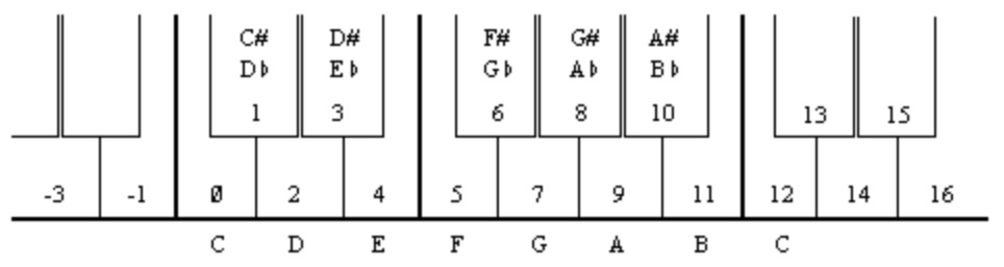
\includegraphics[width=0.7\textwidth]{
                zxspectrumbasicprogramming_pic3
            }
        \end{center}
        \caption{Shema tonov in pripadajočih kod tonov ~\cite{zxspectrumbasicprogramming}.}
        \label{zxspectrumbasicprogramming_pic3}
    \end{figure}

    Na zvočnik lahko poleg ukaza BEEP prek podprogramov ROMa vplivamo tudi z
    ukazi OUT preko V/I vrat \texttt{0xFE}. Bit 4 v podatkovnem zlogu na vratih
    določa stanje zvočnika, pri čemer vrednost 0 pomeni tišino, 1 pa izvajanje
    tona. Ker lahko z enim bitom določamo le stanje proizvajanja zvoka, njegovo
    frekvenco določamo s hitrostjo preklapljanja stanja bita ~\cite{strojnijezikzaprocesorz80}.

    \subsection{Implementacija v emulatorju}

    Zvočni del je vezan na pisanje v V/I vrata \texttt{0xFE}. Vsa pisanja na V/I
    vrata gredo skozi razred \texttt{IOPortSet}, ki zapisano vrednost posreduje
    objektu \texttt{ULABeeper}. Ob vsakem zapisu na V/I vrata \texttt{0xFE} primerja
    trenutno število izvajanih T-stanj procesorja s časom prejšnjega zapisa in iz
    razlike izračuna, koliko vzorcev mora zapisati v zvočni izhod, implementiran z
    neposredno zvočno linijo \texttt{SourceDataLine}. Kadar je bit 4 nastavljen,
    zapisuje vzorce z visoko amplitudo, sicer tišino. S tem se signal zvočnika
    gradi iz istega časovnega modela, ki ga uporablja procesor.

    \chapter{Evalvacija emulatorja}
    \label{evalvacija}

    \subsection{Prikaz delovanja par programov in iger}
    \subsection{Primerjava z obstoječimi emulatorji - hitrost, natančnost}

    \chapter{Zaključek}

    \subsection{Evalvacija uspešnosti diplomskega dela (na podlagi ciljev iz uvoda)}

    \subsection{Možne izboljšave}
    Boljša emulacija časovnih ciklov s strani pomnilnika, procesorja in ULA za
    boljšo sinhronizacijo in emulacijo strojnih napak dejanskega Spectruma: - 1. Memory
    contention - fetching instructions and other general memory reads/writes - I/O
    contention - Port \texttt{0xFE} (ULA port) contention based on address bus
    high byte - Snow effect

    Raje bi uporabil kaj drugega kot KMP, ker cross-platform funkcionalnosti po
    mojem mnenju niso uporabne za razhroščevalnik (kar je glavna komponenta tega projekta),
    prav tako je KMP za desktop privzeto bolj omejen tako v funkcionalnostih kot preformanceu
    (moral iti nivo nižje od KMP za kaj takega). Tako bi razmišljal o drugih
    frameworkih, kot so Electron + TS ali Dioxus/Tauri + Rust.

    %\cleardoublepage
    %\addcontentsline{toc}{chapter}{Literatura}

    % če imaš težave poravnati desni rob bibliografije, potem odkomentiraj spodnjo vrstico
    \raggedright

    \printbibliography
    [heading=bibintoc,type=article,title={Članki v revijah}]

    \printbibliography
    [heading=bibintoc,type=inproceedings,title={Članki v zbornikih}]

    \printbibliography
    [heading=bibintoc,type=incollection,title={Poglavja v knjigah}]

    % v zadnji verziji diplomskega dela običajno združiš vse tri vrste referenc v en sam seznam in
    % izpustiš delne sezname
    \printbibliography
    [heading=bibintoc,title={Literatura}]
\end{document}